\chapter{Primary \texorpdfstring{\Mbc}{Mbc} fits determining initialisation values}\label{sec:appendix_primary_fits}
Before performing an \Mbc fit on the total dataset, the \PDF{s} are defined and prefitted on the individual components, corresponding to the good tag-\B mesons, combinatorial \BB background and continuum background (see \Cref{sec:fitting_components} for definitions).
The \Mbc fits on each \EB bi (see \Cref{sec:binning}) for the aforementioned components of the dataset are provided in this Chapter.
The fits are as follows:
\begin{itemize}
    \item Crystal Ball \PDF fits, on the good tag-\B \Mbc distribution (\Cref{fig:primary_cb_fits}).
    \item ARGUS\PDF fits, on the continuum event \Mbc distribution (\Cref{fig:primary_argus_fits}).
    \item Chebyshev \PDF fits, on the combinatorial \BB tag bacgkground distribution (\Cref{fig:primary_cheb_fits}).
\end{itemize}

Additionally, the ARGUS and Chebyshev \PDF{s} are combined together after fitting, to show that a good overall description of background (other than good tag-\B counts) is achieved.
This is shown in  \Cref{fig:primary_bkg_fits}.

Although small innacuracies of the fitter may be spotted (e.g. $2.4-2.6~\gev$ region in \Cref{fig:primary_cheb_fits}) The primary goals of the fitter is to describe the Crystal Ball normalisation parameter.
Moreover, these fits are prepared on 1.6~\invab, whereas the measurement is planned on a dataset roughly one order of magnitude smaller.
Therefore, at this stage, such description preforms sufficiently well for the goal of the analysis.

\begin{figure}[htbp!]
    \centering
    \subcaptionbox{\label{fig:mbc_crys_1p4}}{
        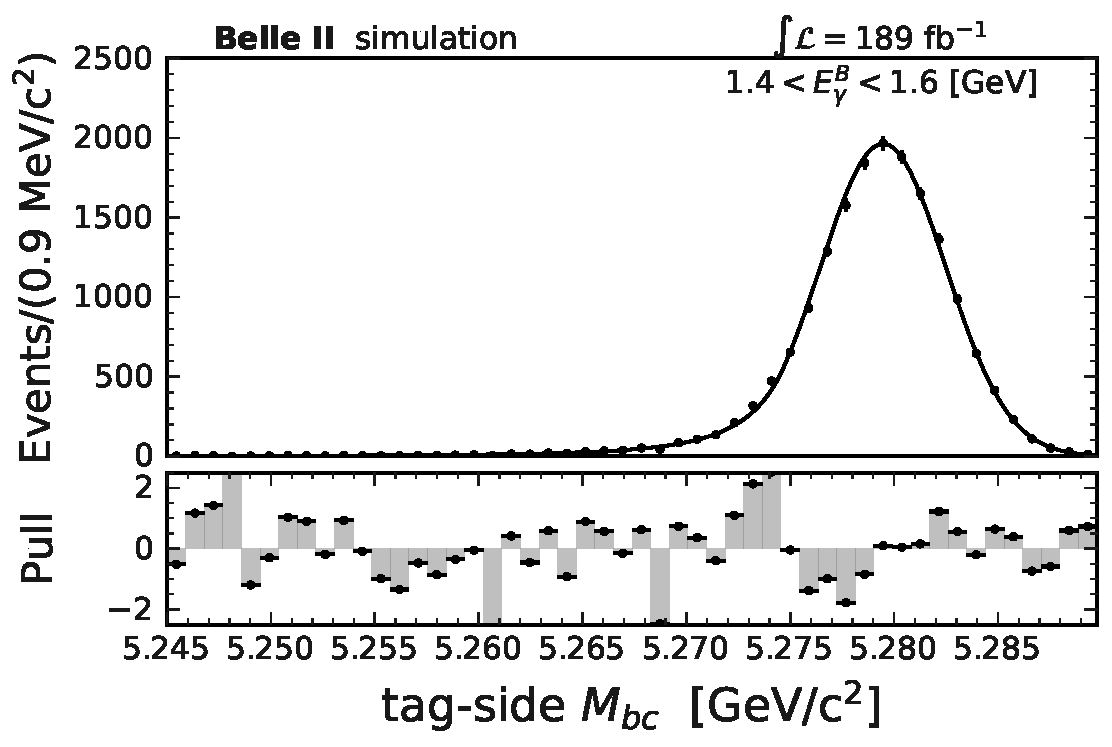
\includegraphics[width=0.3\textwidth]{figures/appendices/primary_fits/CB_MbcFit_1p4to1p6ppdf.pdf}
    }
    \subcaptionbox{\label{fig:mbc_crys_1p6}}{
        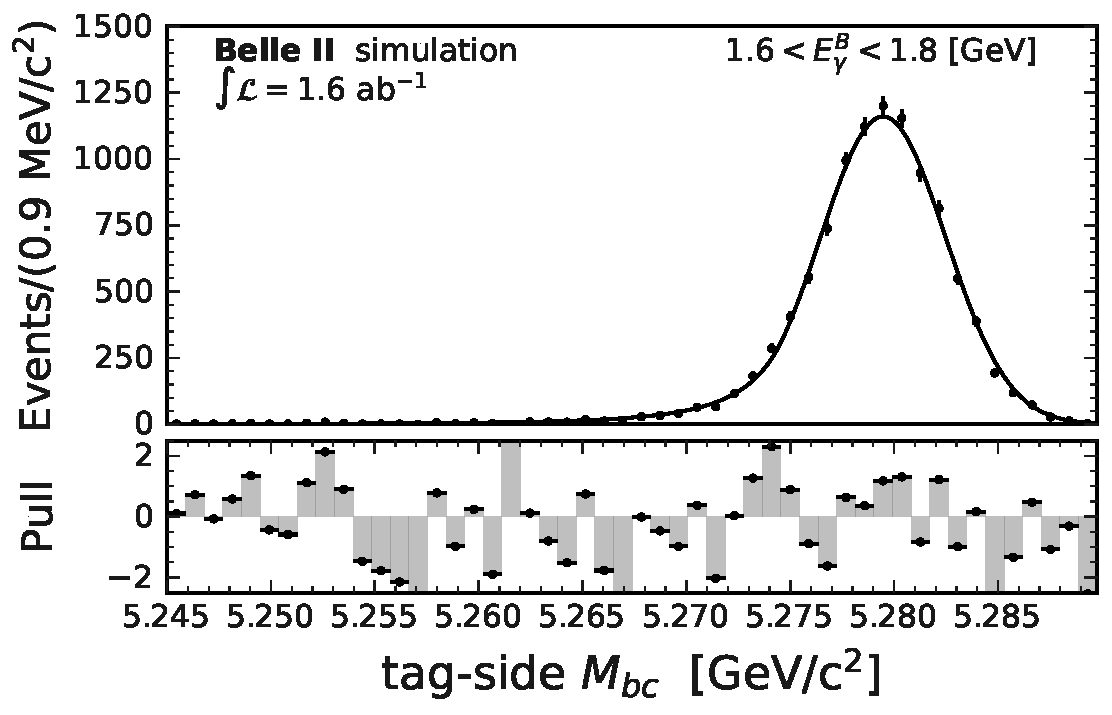
\includegraphics[width=0.3\textwidth]{figures/appendices/primary_fits/CB_MbcFit_1p6to1p8ppdf.pdf}
    }
    \subcaptionbox{\label{fig:mbc_crys_1p8}}{
        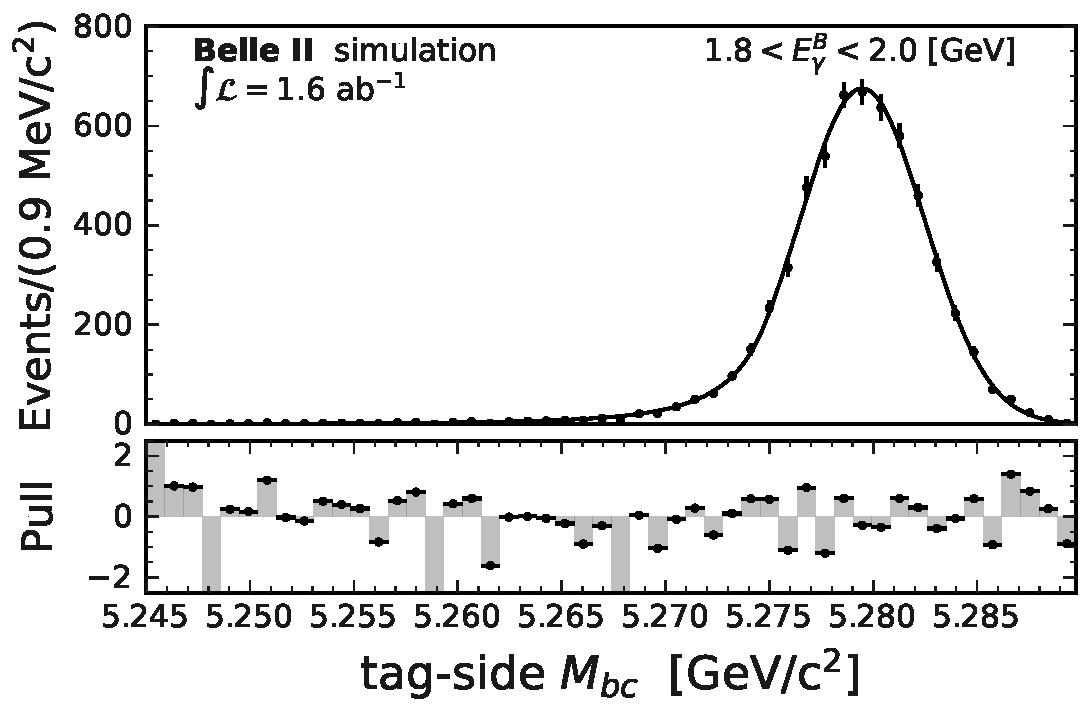
\includegraphics[width=0.3\textwidth]{figures/appendices/primary_fits/CB_MbcFit_1p8to2p0ppdf.pdf}
    }
    \subcaptionbox{\label{fig:mbc_crys_2p0}}{
        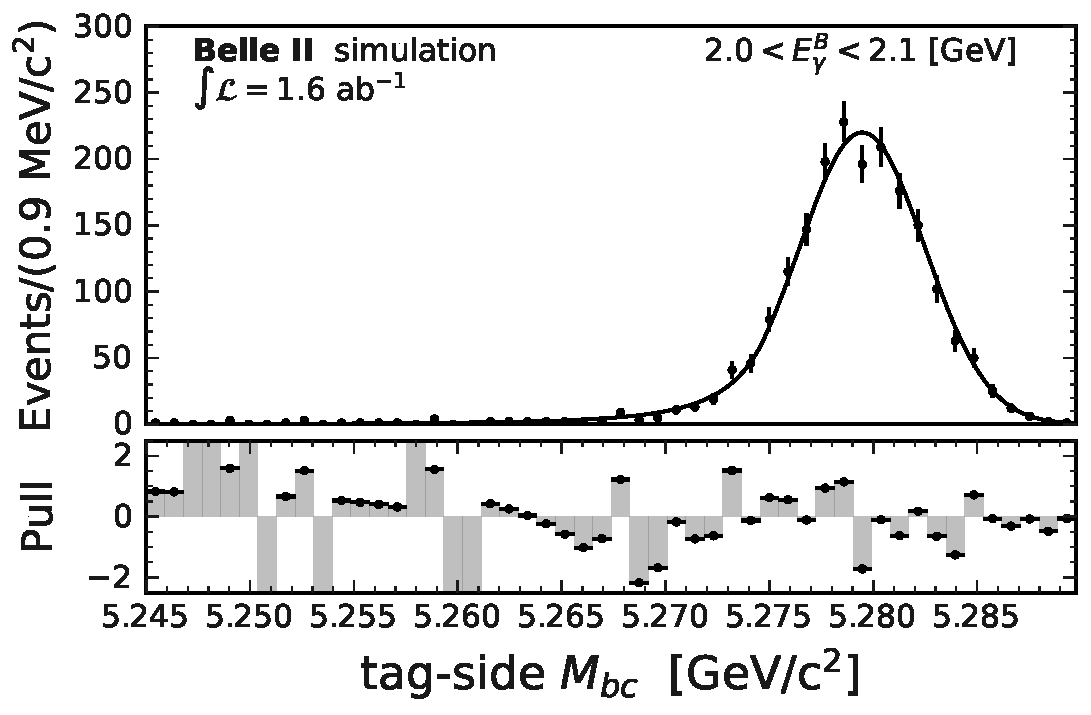
\includegraphics[width=0.3\textwidth]{figures/appendices/primary_fits/CB_MbcFit_2p0to2p1ppdf.pdf}
    }
    \subcaptionbox{\label{fig:mbc_crys_2p1}}{
        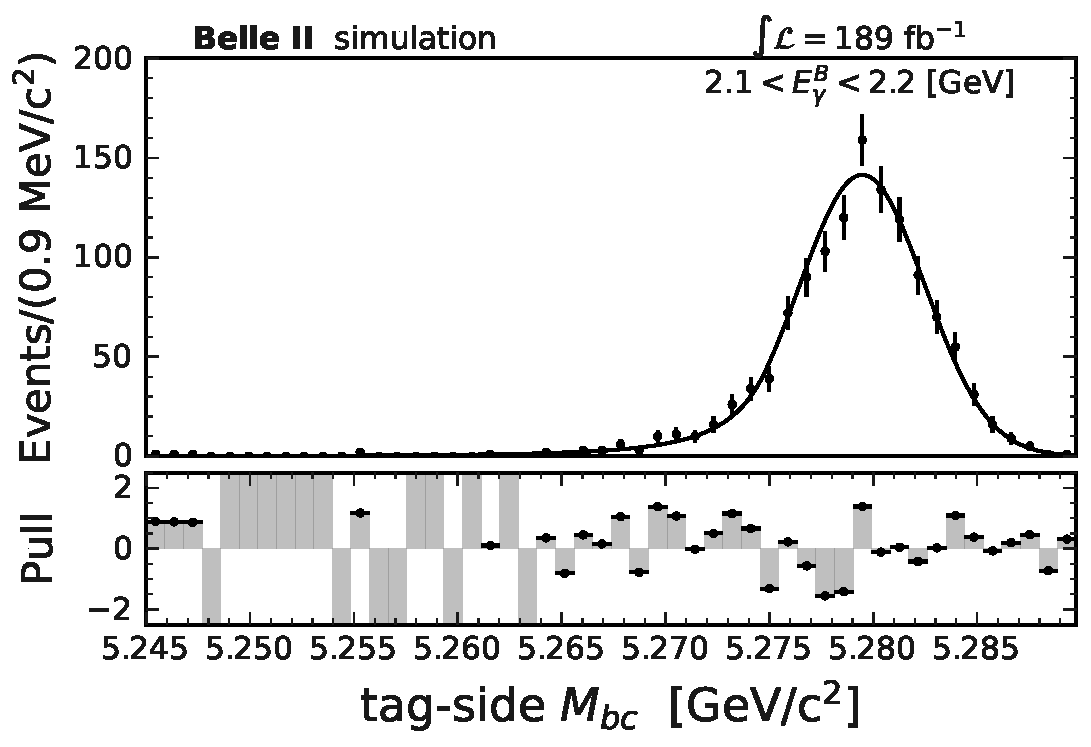
\includegraphics[width=0.3\textwidth]{figures/appendices/primary_fits/CB_MbcFit_2p1to2p2ppdf.pdf}
    }
    \subcaptionbox{\label{fig:mbc_crys_2p2}}{
        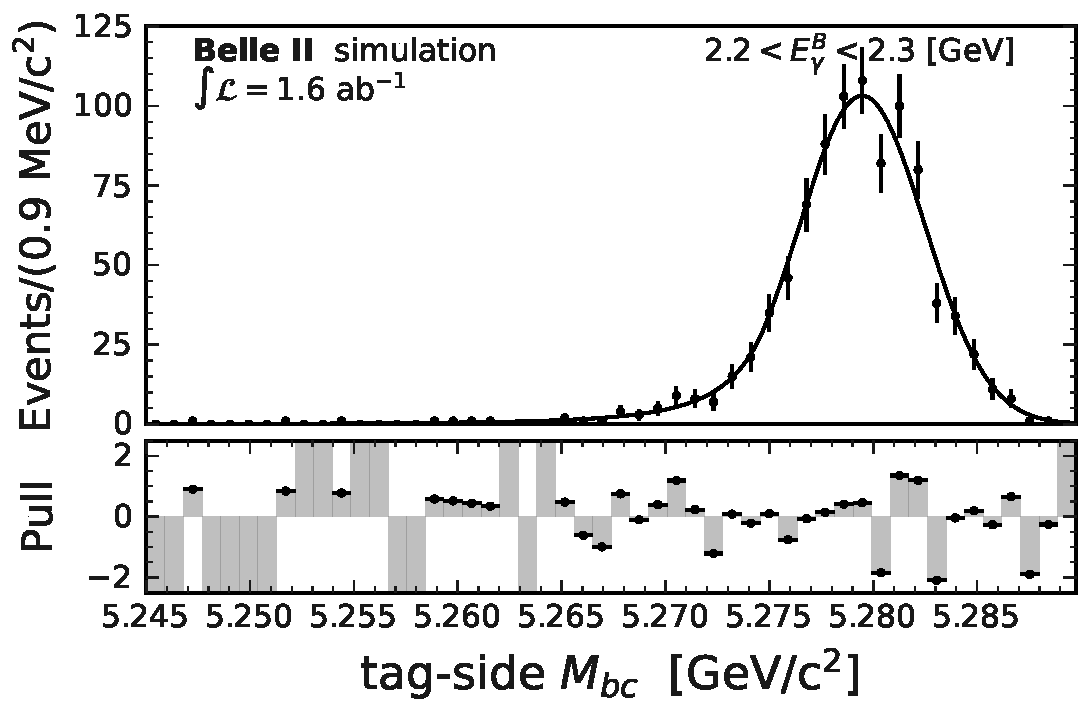
\includegraphics[width=0.3\textwidth]{figures/appendices/primary_fits/CB_MbcFit_2p2to2p3ppdf.pdf}
    }
    \subcaptionbox{\label{fig:mbc_crys_2p3}}{
        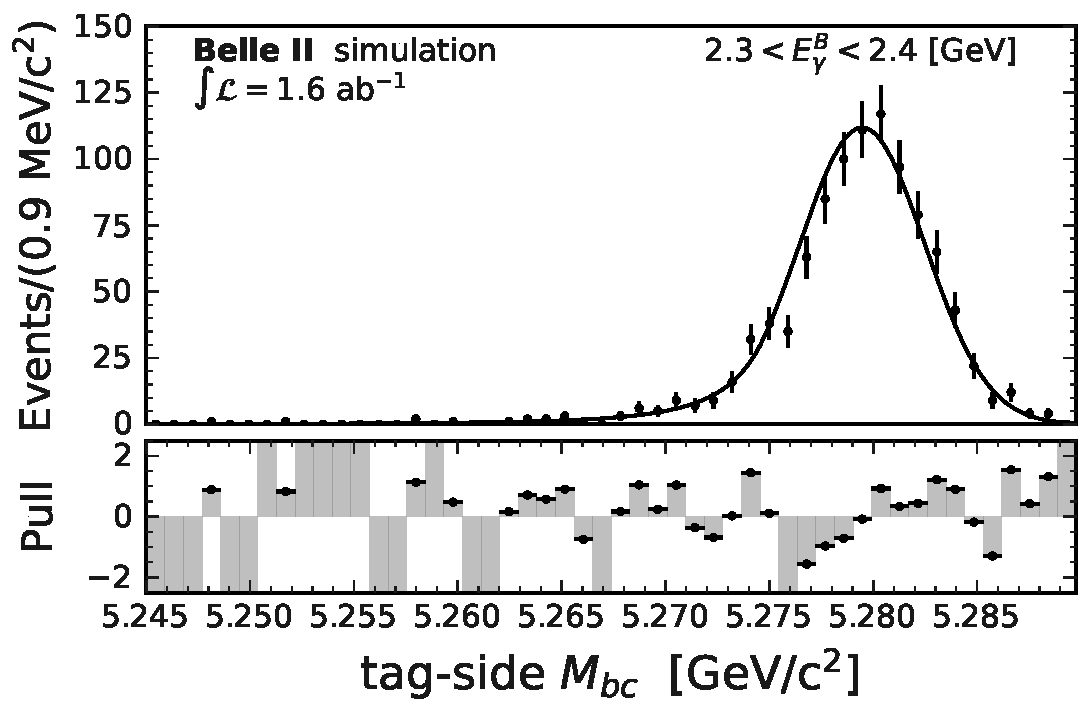
\includegraphics[width=0.3\textwidth]{figures/appendices/primary_fits/CB_MbcFit_2p3to2p4ppdf.pdf}
    }
    \subcaptionbox{\label{fig:mbc_crys_2p4}}{
        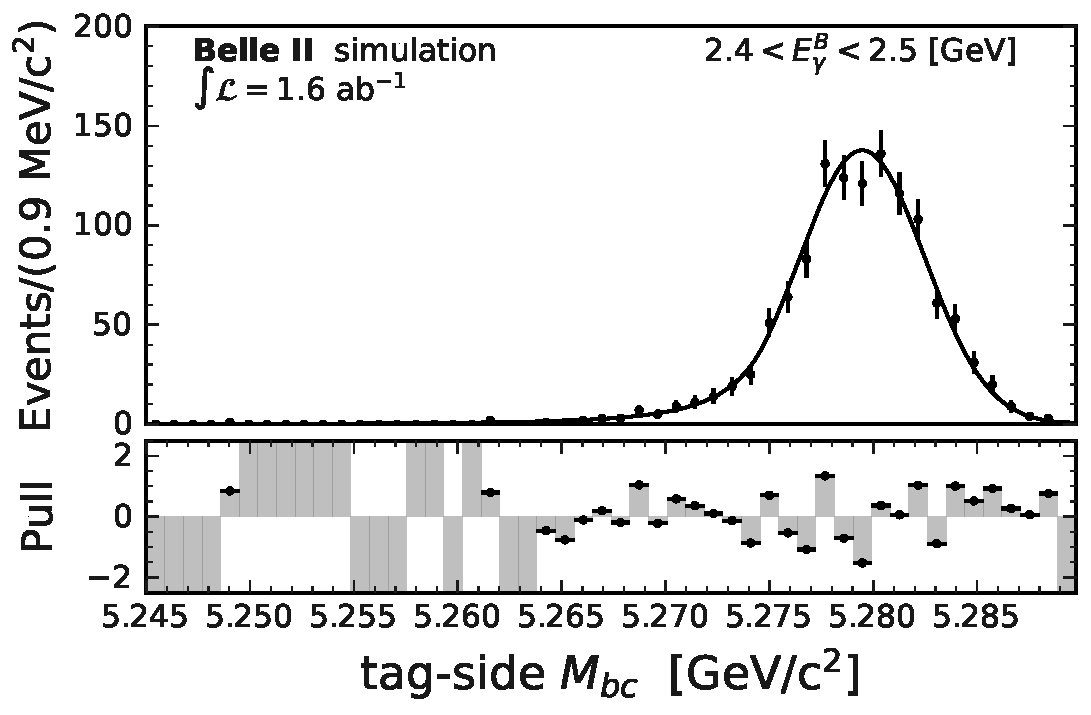
\includegraphics[width=0.3\textwidth]{figures/appendices/primary_fits/CB_MbcFit_2p4to2p5ppdf.pdf}
    }
    \subcaptionbox{\label{fig:mbc_crys_2p5}}{
        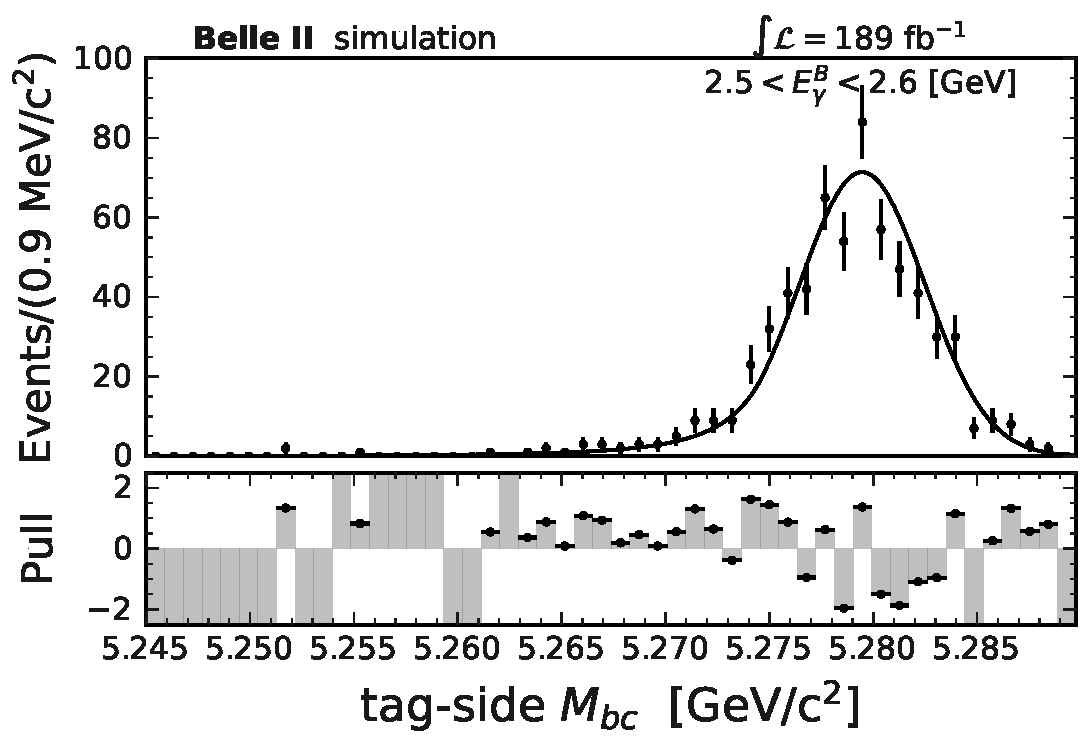
\includegraphics[width=0.3\textwidth]{figures/appendices/primary_fits/CB_MbcFit_2p5to2p6ppdf.pdf}
    }
    \subcaptionbox{\label{fig:mbc_crys_2p6}}{
        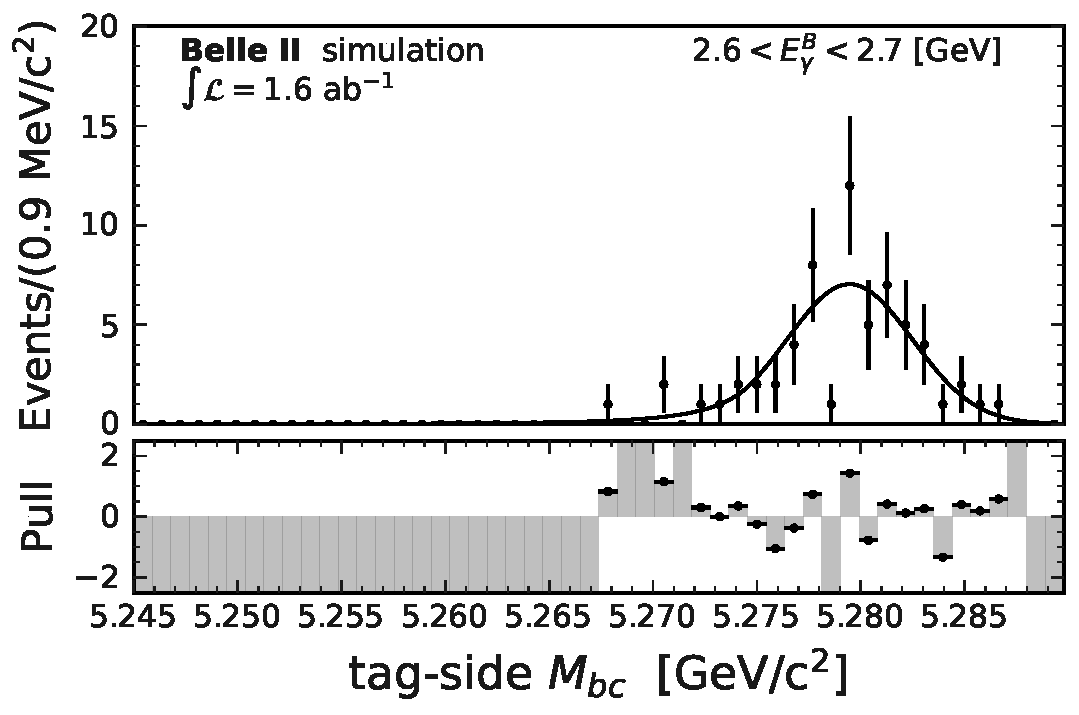
\includegraphics[width=0.3\textwidth]{figures/appendices/primary_fits/CB_MbcFit_2p6to2p7ppdf.pdf}
    }
    \subcaptionbox{\label{fig:mbc_crys_2p7}}{
        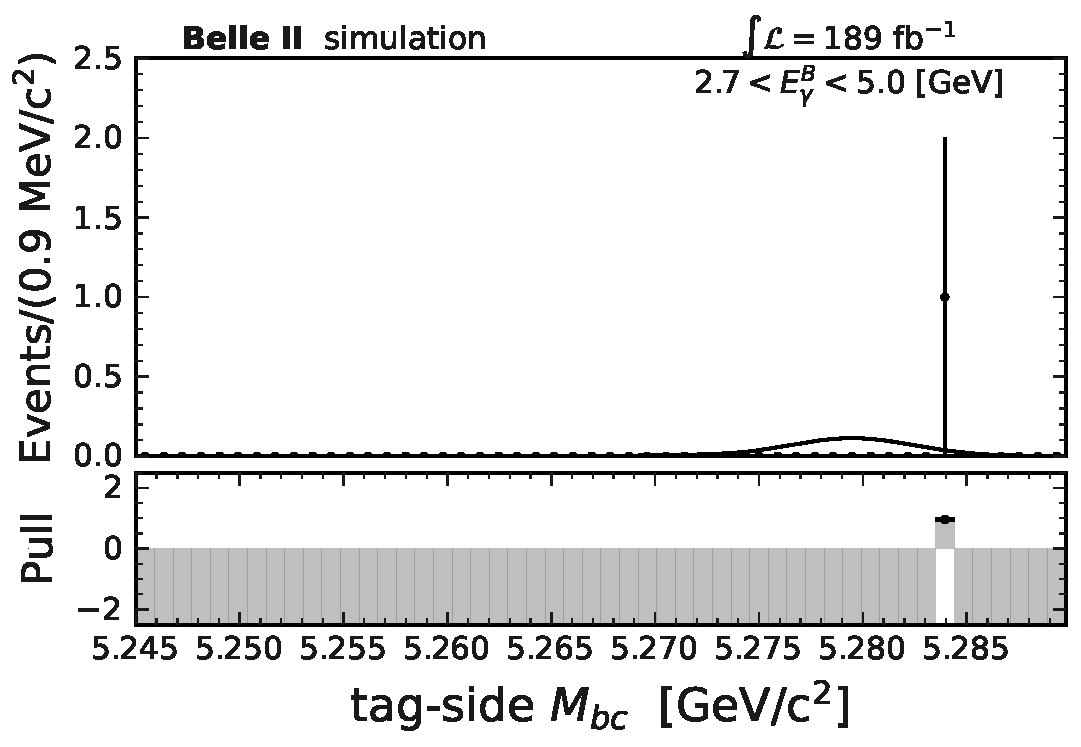
\includegraphics[width=0.3\textwidth]{figures/appendices/primary_fits/CB_MbcFit_2p7to5p0ppdf.pdf}
    }
    \caption{\label{fig:primary_cb_fits}The fits on the good tag-\B meson events in generic \MC, using the Crystal Ball \PDF.
    This fit allows to extract initialisation values for further fitting of the total datasets.
    Good description of the \Mbc distributions can be seen throughout the \EB bins.
    }
\end{figure}

\begin{figure}[htbp!]
    \centering
    \subcaptionbox{\label{fig:mbc_argus_1p4}}{
        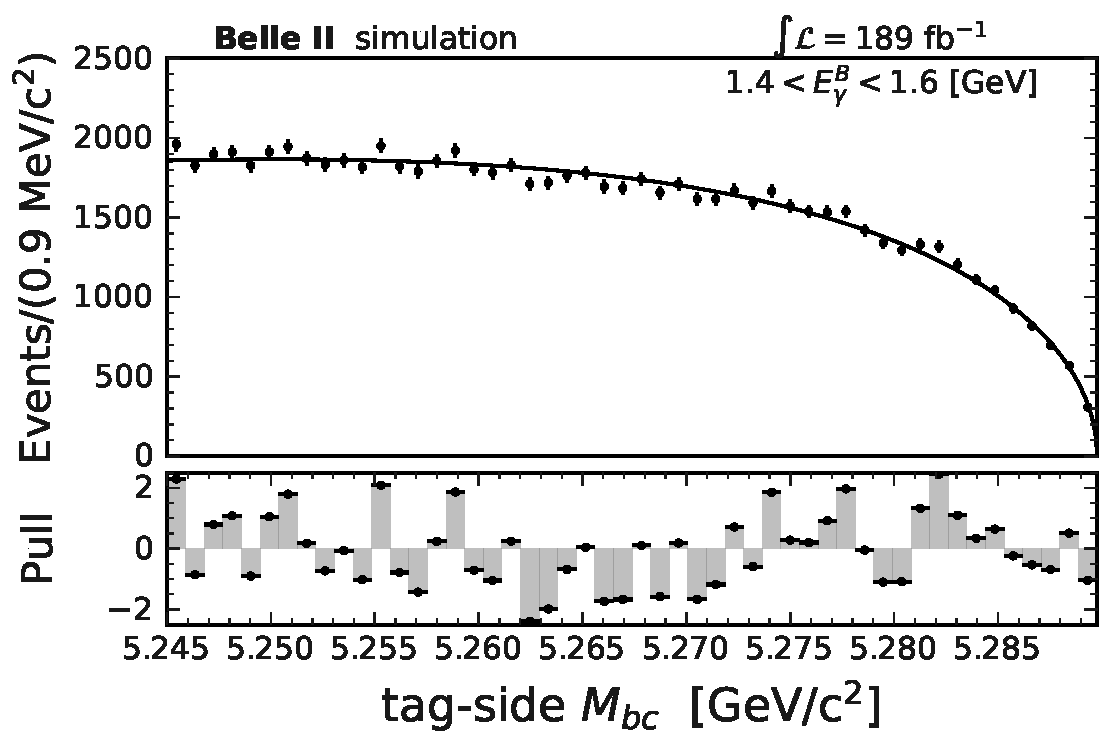
\includegraphics[width=0.3\textwidth]{figures/appendices/primary_fits/ARGUS_MbcFit_1p4to1p6ppdf.pdf}
    }
    \subcaptionbox{\label{fig:mbc_argus_1p6}}{
        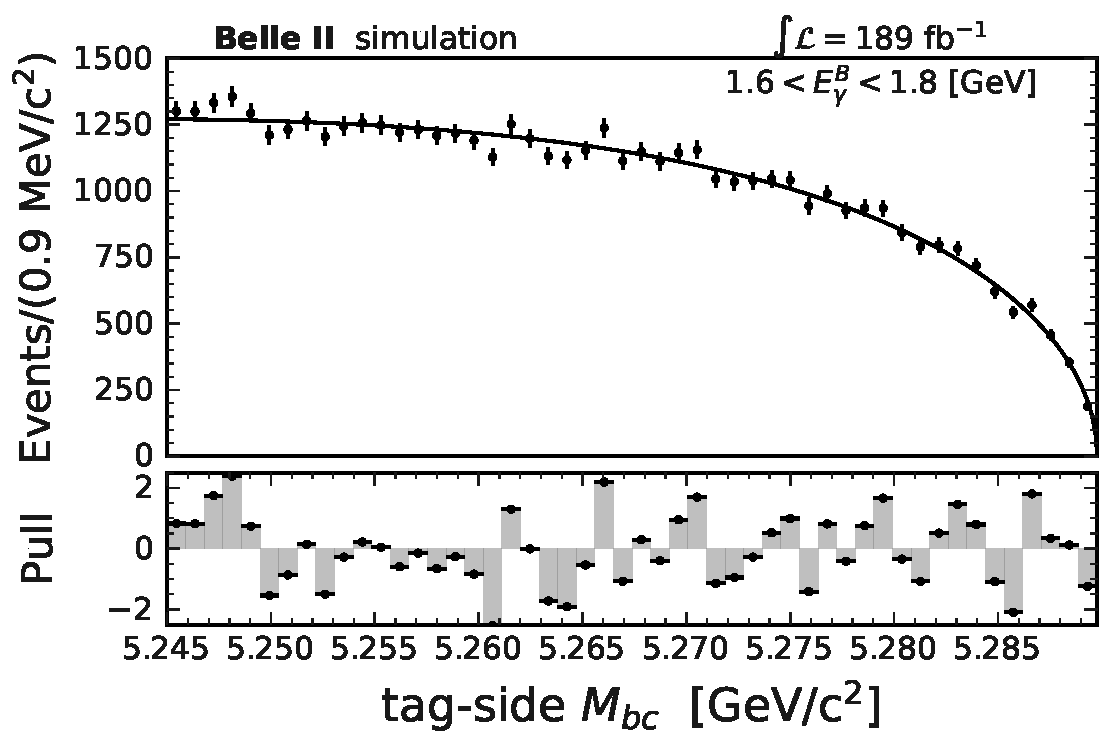
\includegraphics[width=0.3\textwidth]{figures/appendices/primary_fits/ARGUS_MbcFit_1p6to1p8ppdf.pdf}
    }
    \subcaptionbox{\label{fig:mbc_argus_1p8}}{
        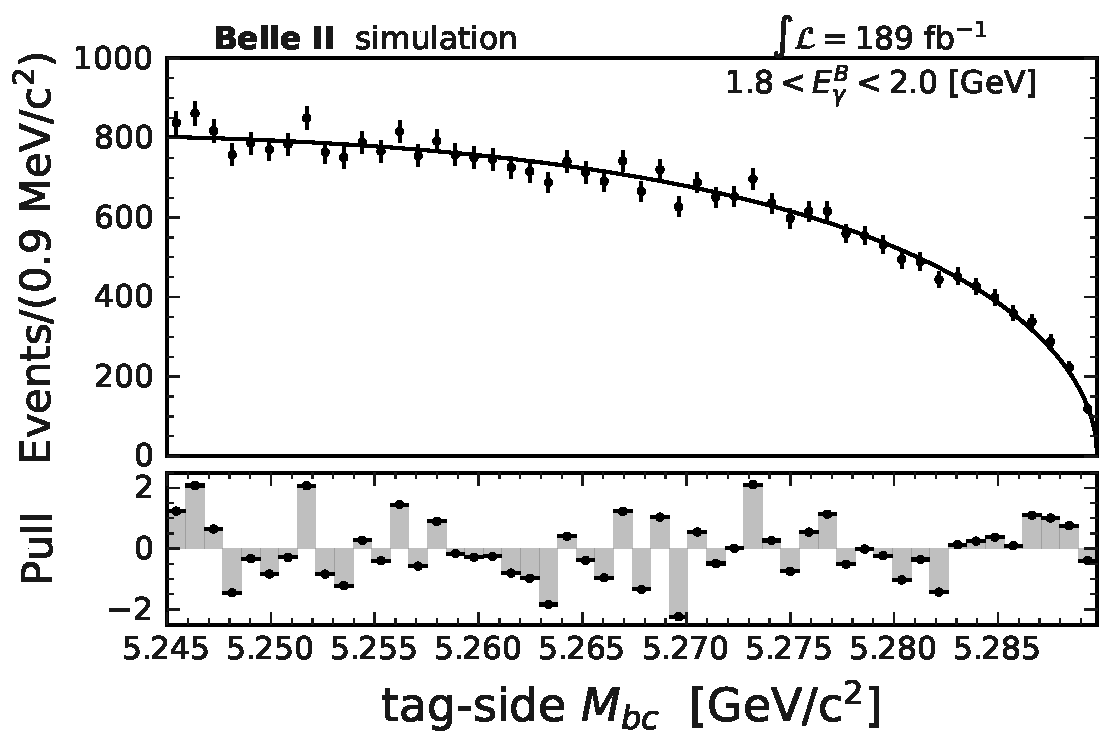
\includegraphics[width=0.3\textwidth]{figures/appendices/primary_fits/ARGUS_MbcFit_1p8to2p0ppdf.pdf}
    }
    \subcaptionbox{\label{fig:mbc_argus_2p0}}{
        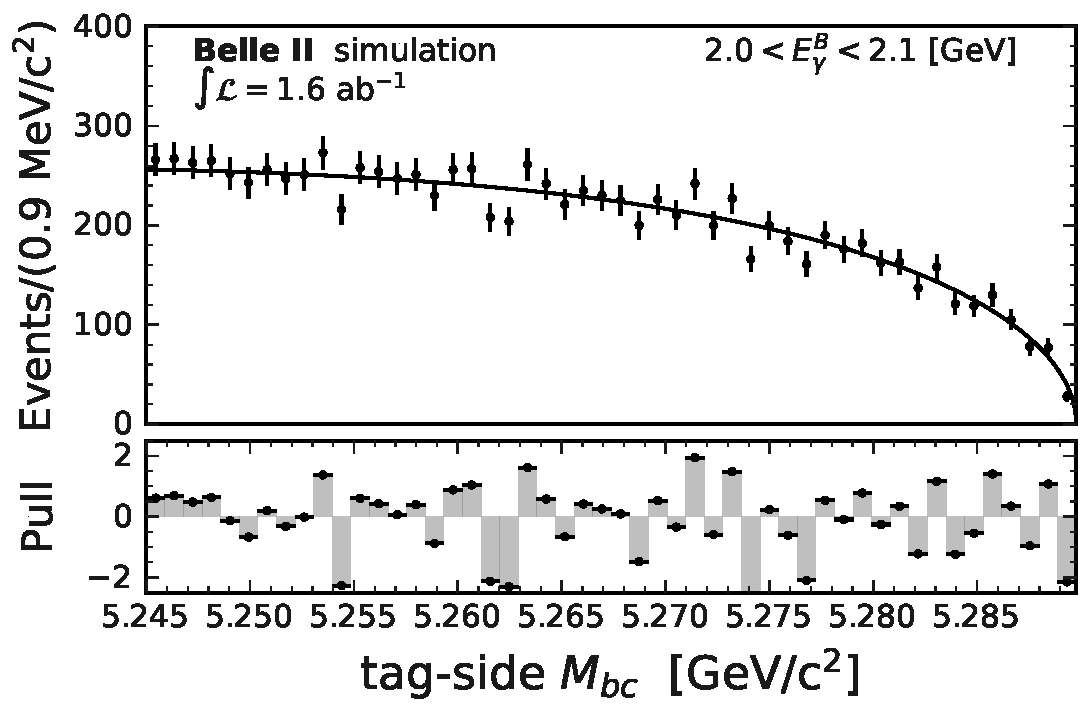
\includegraphics[width=0.3\textwidth]{figures/appendices/primary_fits/ARGUS_MbcFit_2p0to2p1ppdf.pdf}
    }
    \subcaptionbox{\label{fig:mbc_argus_2p1}}{
        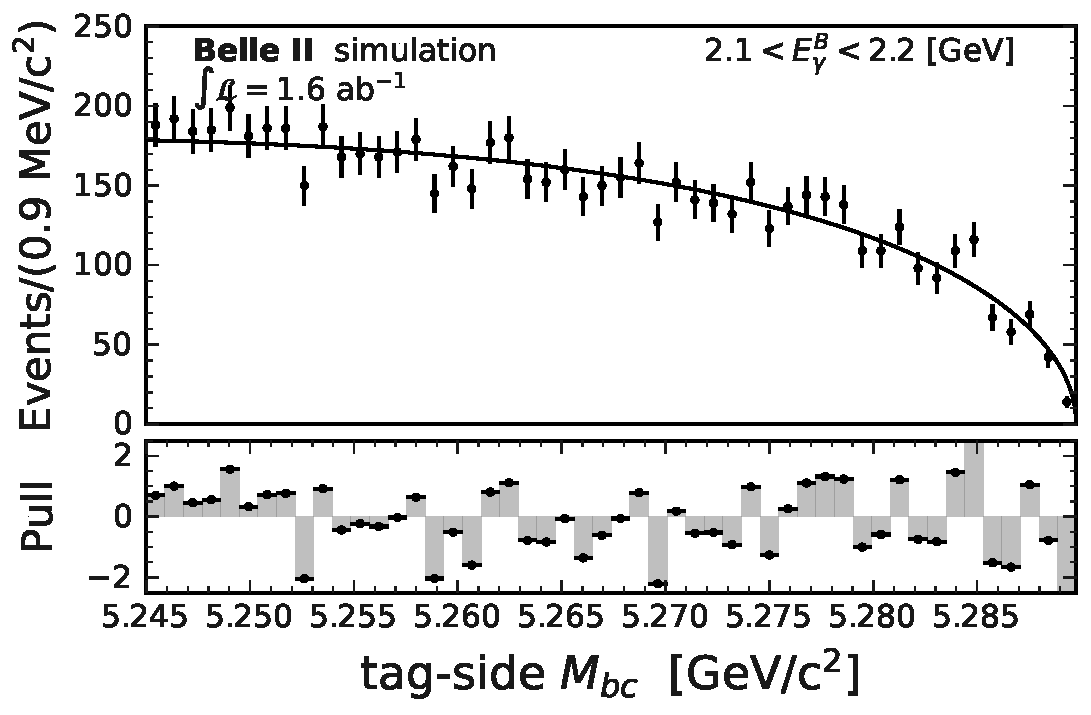
\includegraphics[width=0.3\textwidth]{figures/appendices/primary_fits/ARGUS_MbcFit_2p1to2p2ppdf.pdf}
    }
    \subcaptionbox{\label{fig:mbc_argus_2p2}}{
        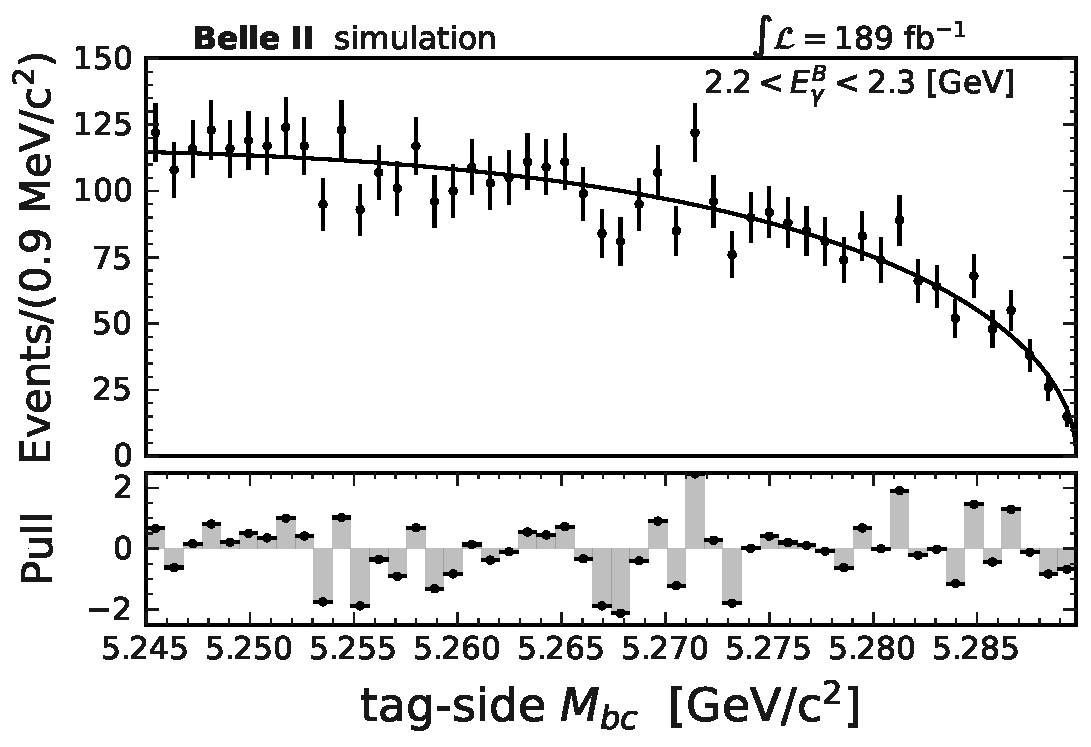
\includegraphics[width=0.3\textwidth]{figures/appendices/primary_fits/ARGUS_MbcFit_2p2to2p3ppdf.pdf}
    }
    \subcaptionbox{\label{fig:mbc_argus_2p3}}{
        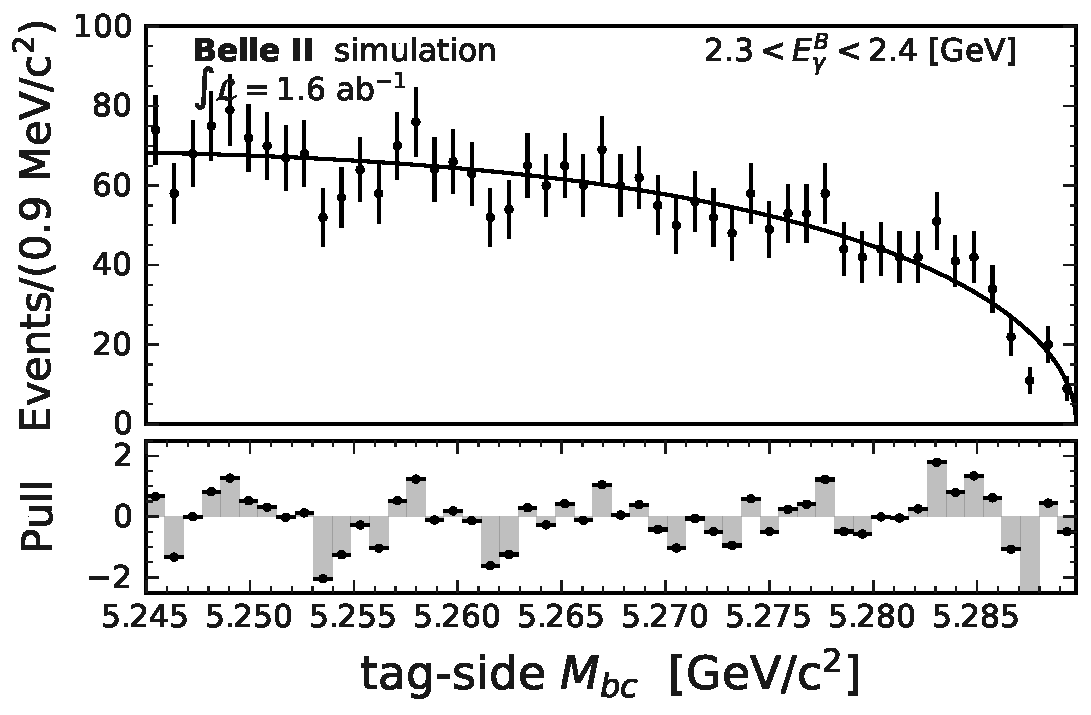
\includegraphics[width=0.3\textwidth]{figures/appendices/primary_fits/ARGUS_MbcFit_2p3to2p4ppdf.pdf}
    }
    \subcaptionbox{\label{fig:mbc_argus_2p4}}{
        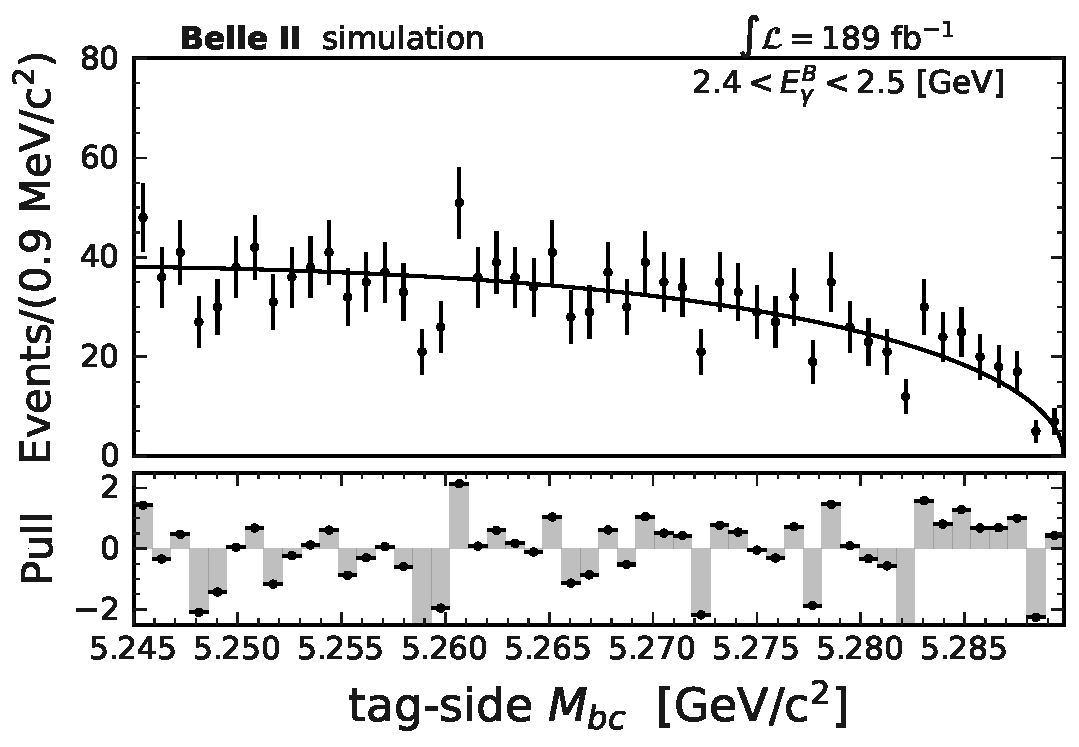
\includegraphics[width=0.3\textwidth]{figures/appendices/primary_fits/ARGUS_MbcFit_2p4to2p5ppdf.pdf}
    }
    \subcaptionbox{\label{fig:mbc_argus_2p5}}{
        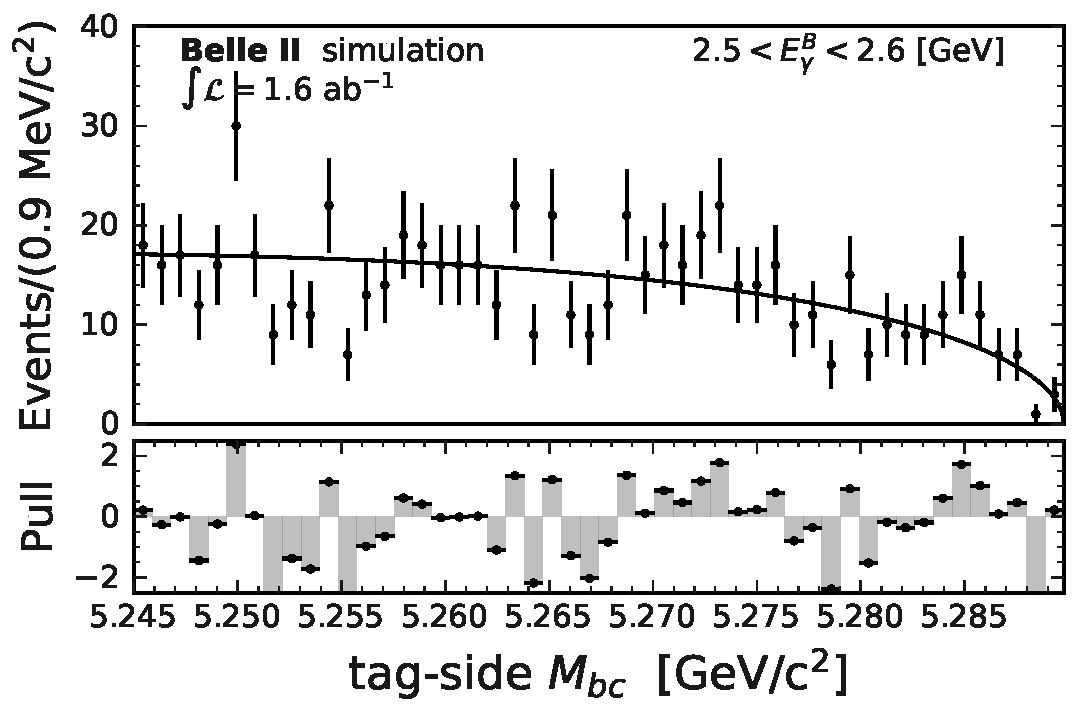
\includegraphics[width=0.3\textwidth]{figures/appendices/primary_fits/ARGUS_MbcFit_2p5to2p6ppdf.pdf}
    }
    \subcaptionbox{\label{fig:mbc_argus_2p6}}{
        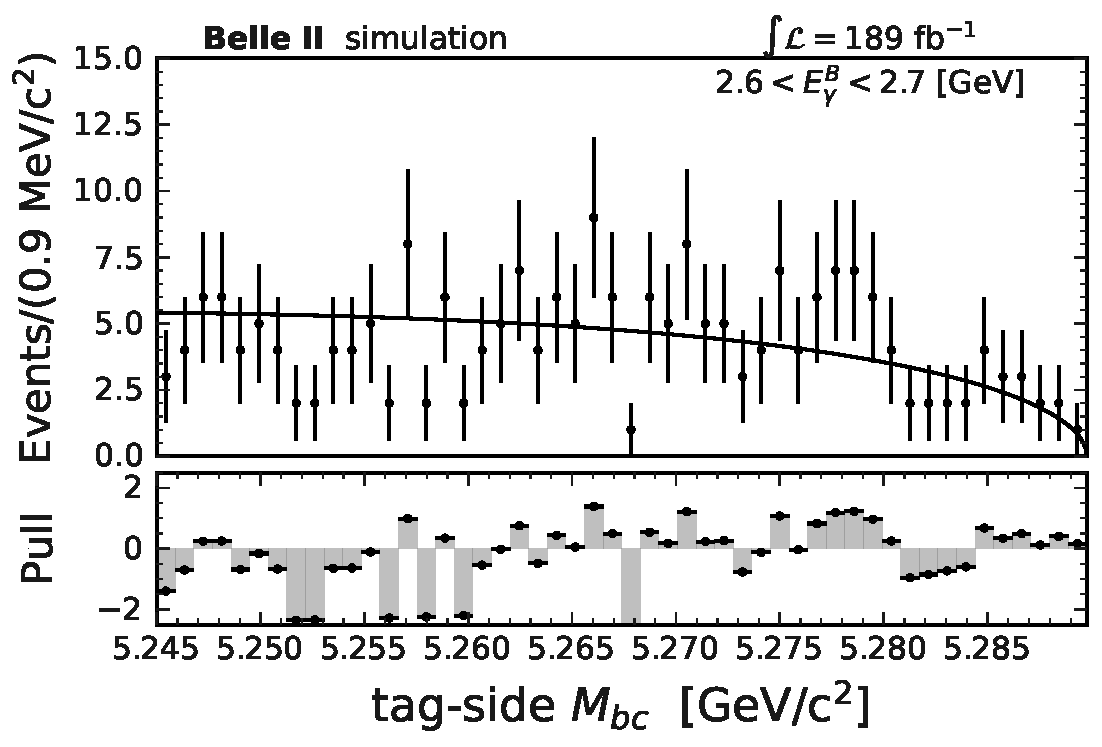
\includegraphics[width=0.3\textwidth]{figures/appendices/primary_fits/ARGUS_MbcFit_2p6to2p7ppdf.pdf}
    }
    \subcaptionbox{\label{fig:mbc_argus_2p7}}{
        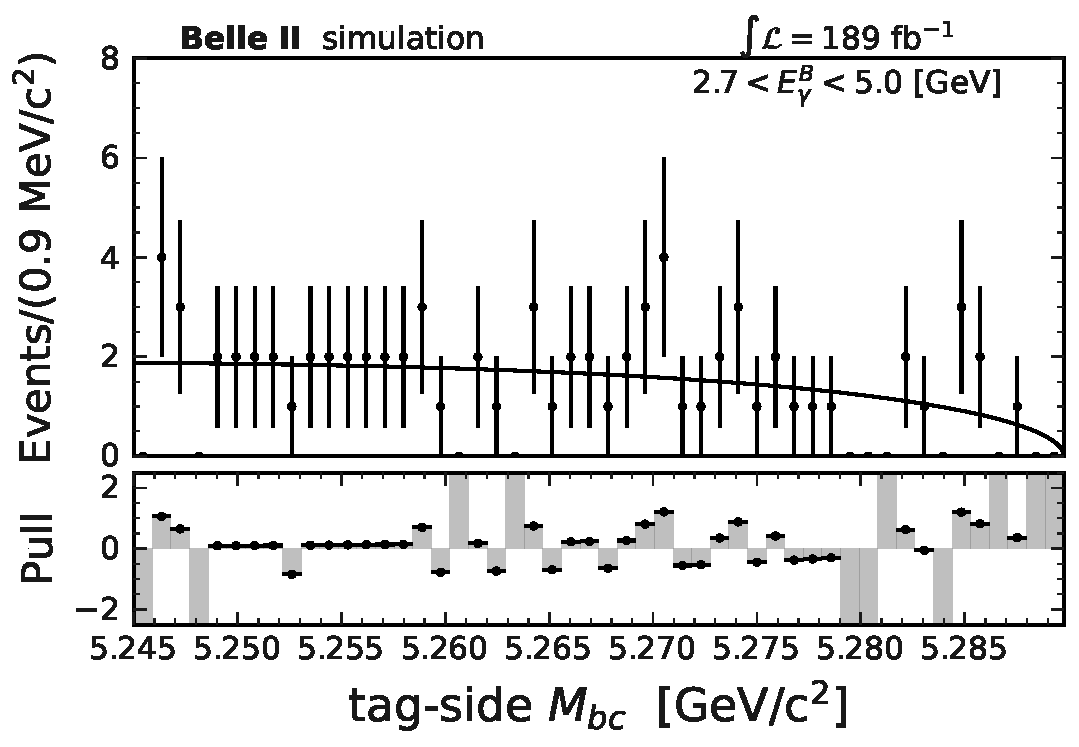
\includegraphics[width=0.3\textwidth]{figures/appendices/primary_fits/ARGUS_MbcFit_2p7to5p0ppdf.pdf}
    }
    \caption{\label{fig:primary_argus_fits}The fits on the continuum events in generic \MC, using the ARGUS \PDF.
    This fit allows to extract initialisation values for further fitting of the total datasets.
    Good description of the \Mbc distributions can be seen throughout the \EB bins.
    }
\end{figure}

\begin{figure}[htbp!]
    \centering
    \subcaptionbox{\label{fig:mbc_cheb_1p4}}{
        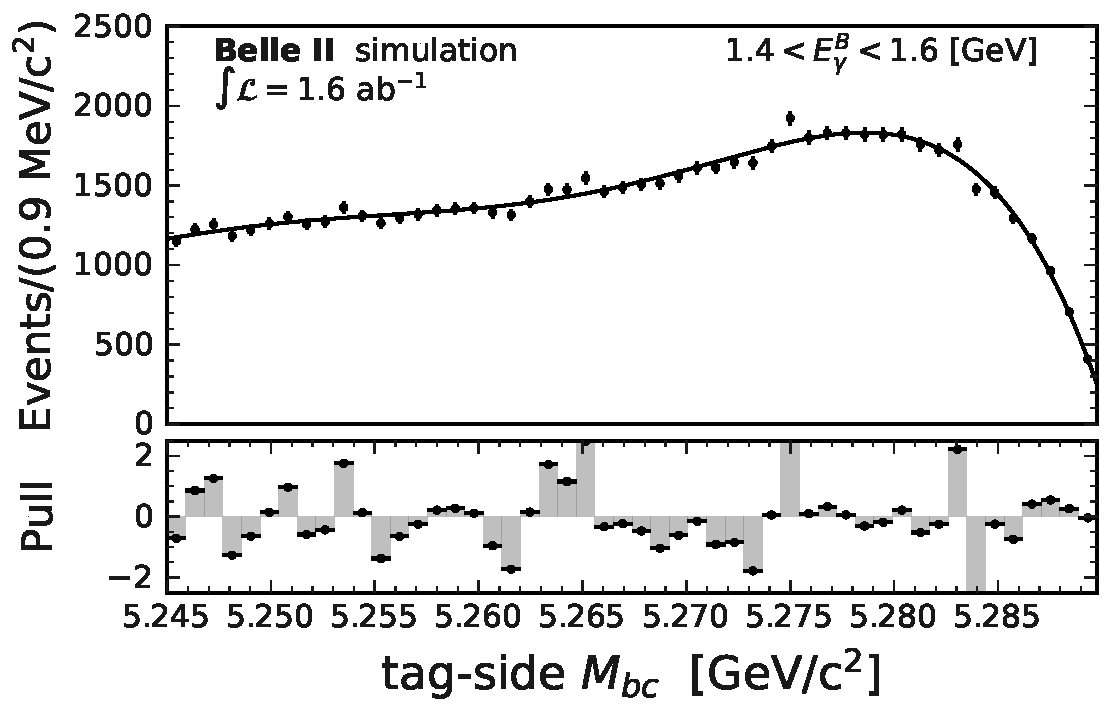
\includegraphics[width=0.3\textwidth]{figures/appendices/primary_fits/CHEB_MbcFit_1p4to1p6ppdf.pdf}
    }
    \subcaptionbox{\label{fig:mbc_cheb_1p6}}{
        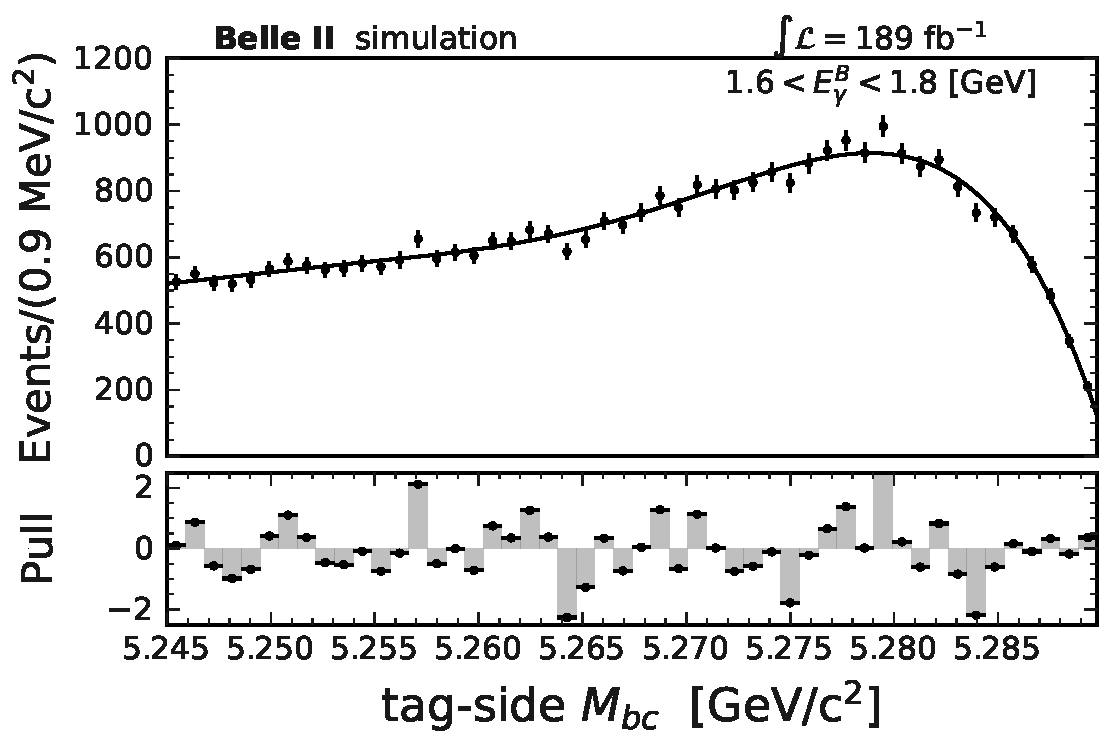
\includegraphics[width=0.3\textwidth]{figures/appendices/primary_fits/CHEB_MbcFit_1p6to1p8ppdf.pdf}
    }
    \subcaptionbox{\label{fig:mbc_cheb_1p8}}{
        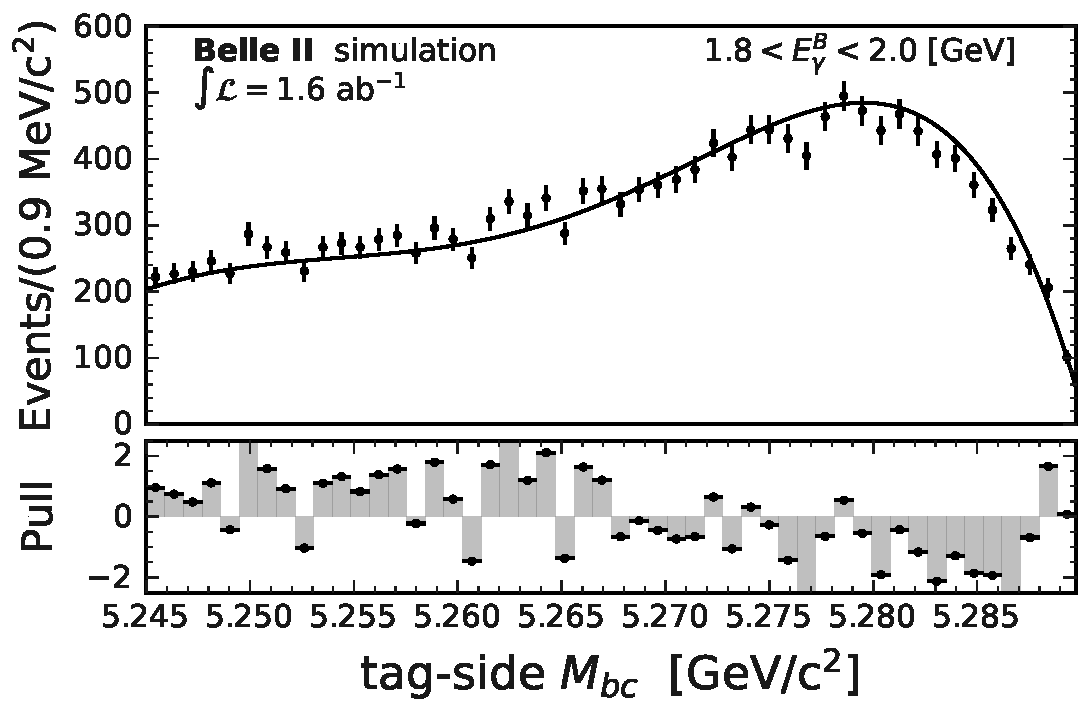
\includegraphics[width=0.3\textwidth]{figures/appendices/primary_fits/CHEB_MbcFit_1p8to2p0ppdf.pdf}
    }
    \subcaptionbox{\label{fig:mbc_cheb_2p0}}{
        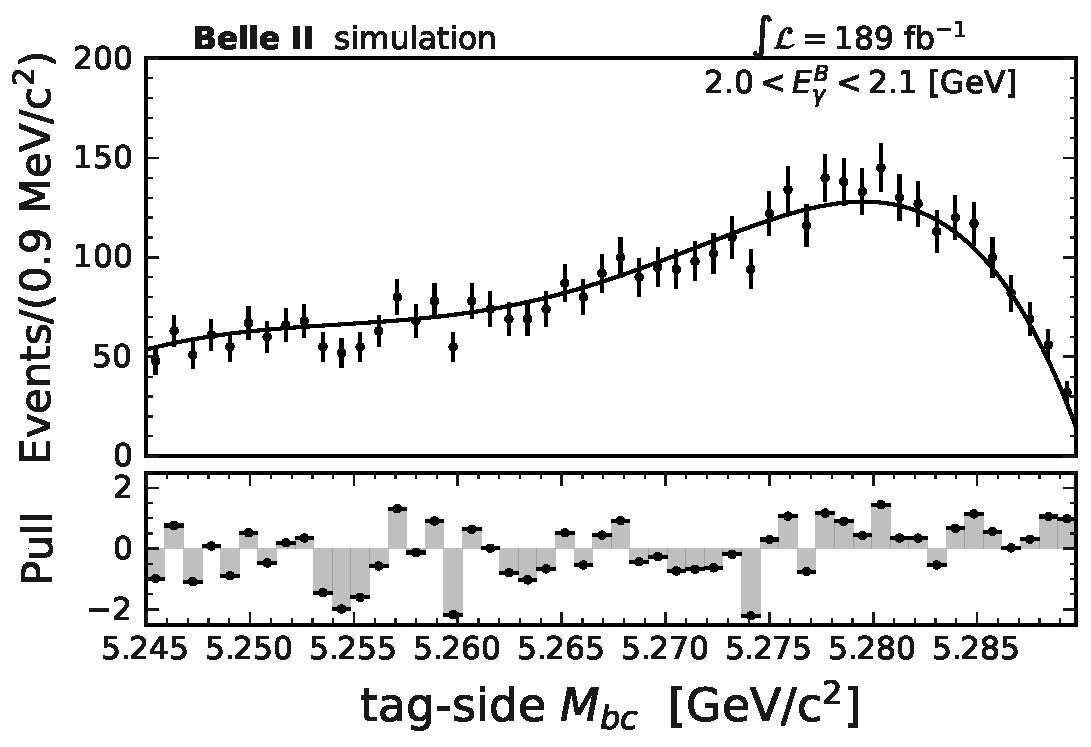
\includegraphics[width=0.3\textwidth]{figures/appendices/primary_fits/CHEB_MbcFit_2p0to2p1ppdf.pdf}
    }
    \subcaptionbox{\label{fig:mbc_cheb_2p1}}{
        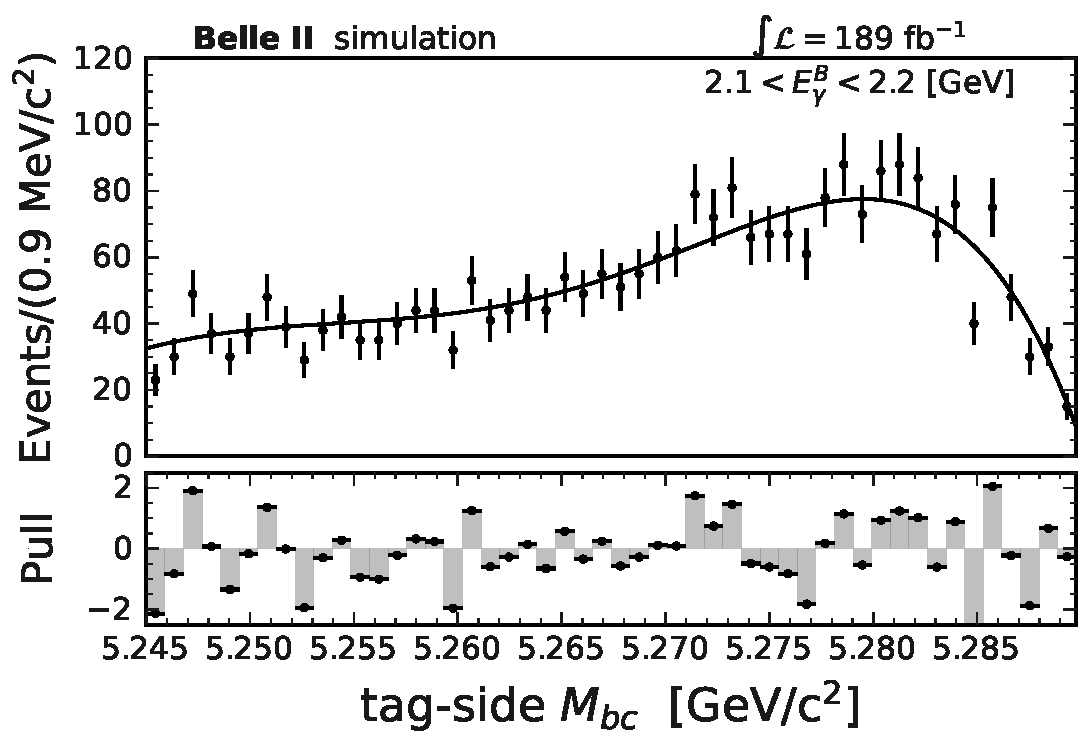
\includegraphics[width=0.3\textwidth]{figures/appendices/primary_fits/CHEB_MbcFit_2p1to2p2ppdf.pdf}
    }
    \subcaptionbox{\label{fig:mbc_cheb_2p2}}{
        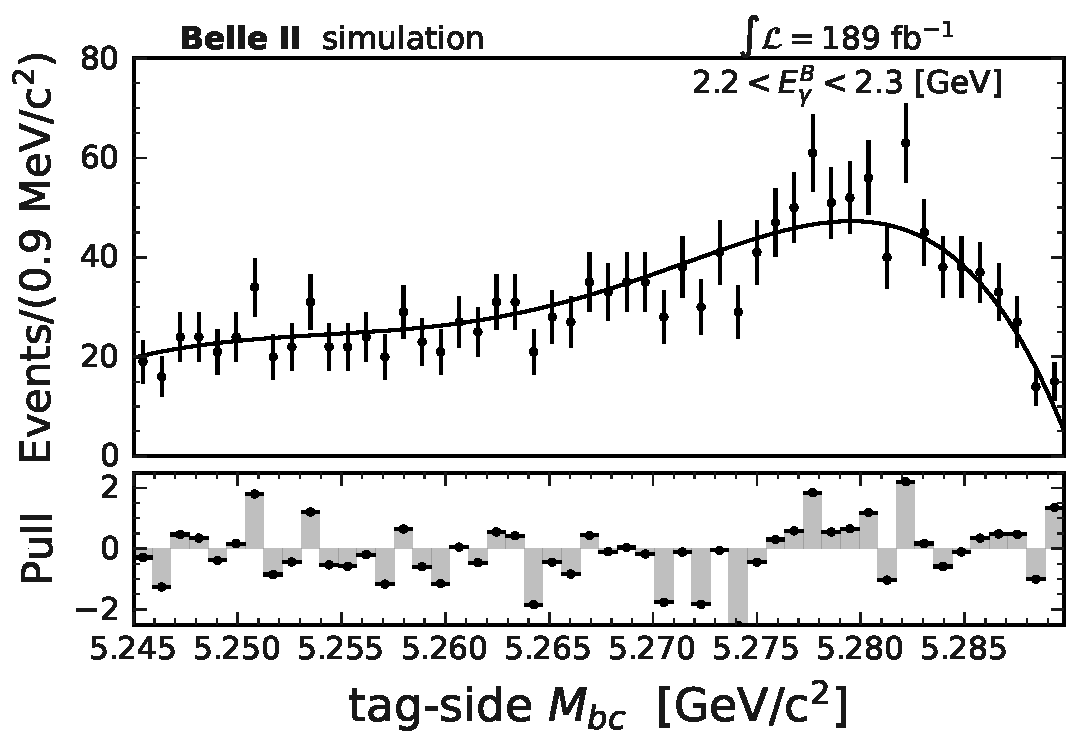
\includegraphics[width=0.3\textwidth]{figures/appendices/primary_fits/CHEB_MbcFit_2p2to2p3ppdf.pdf}
    }
    \subcaptionbox{\label{fig:mbc_cheb_2p3}}{
        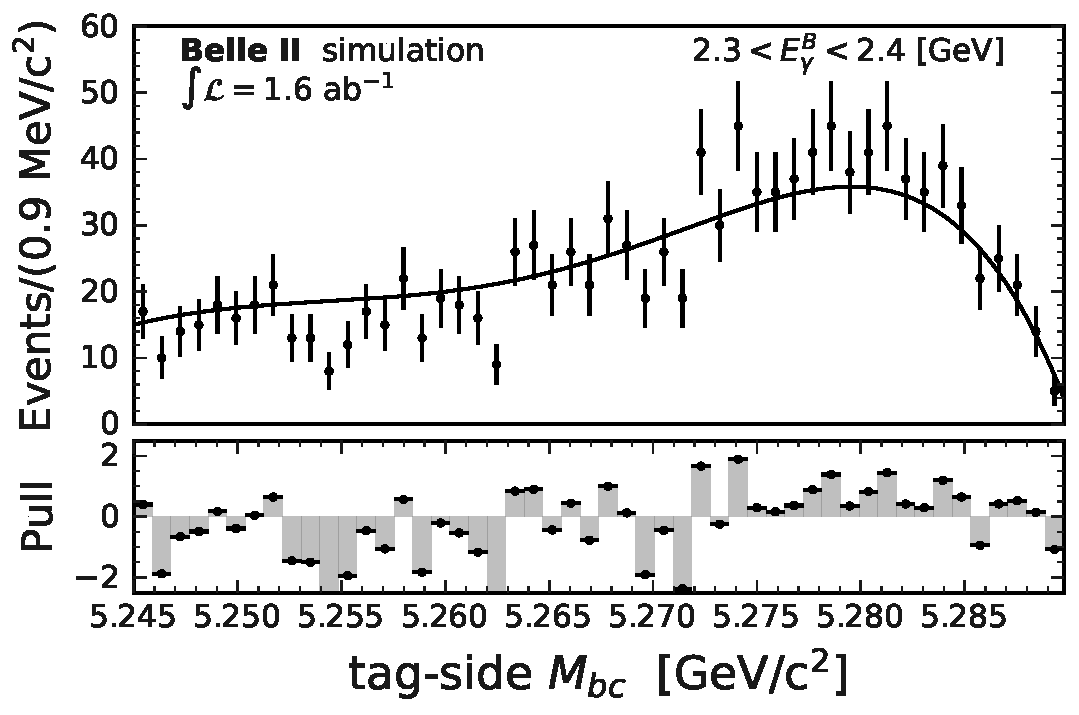
\includegraphics[width=0.3\textwidth]{figures/appendices/primary_fits/CHEB_MbcFit_2p3to2p4ppdf.pdf}
    }
    \subcaptionbox{\label{fig:mbc_cheb_2p4}}{
        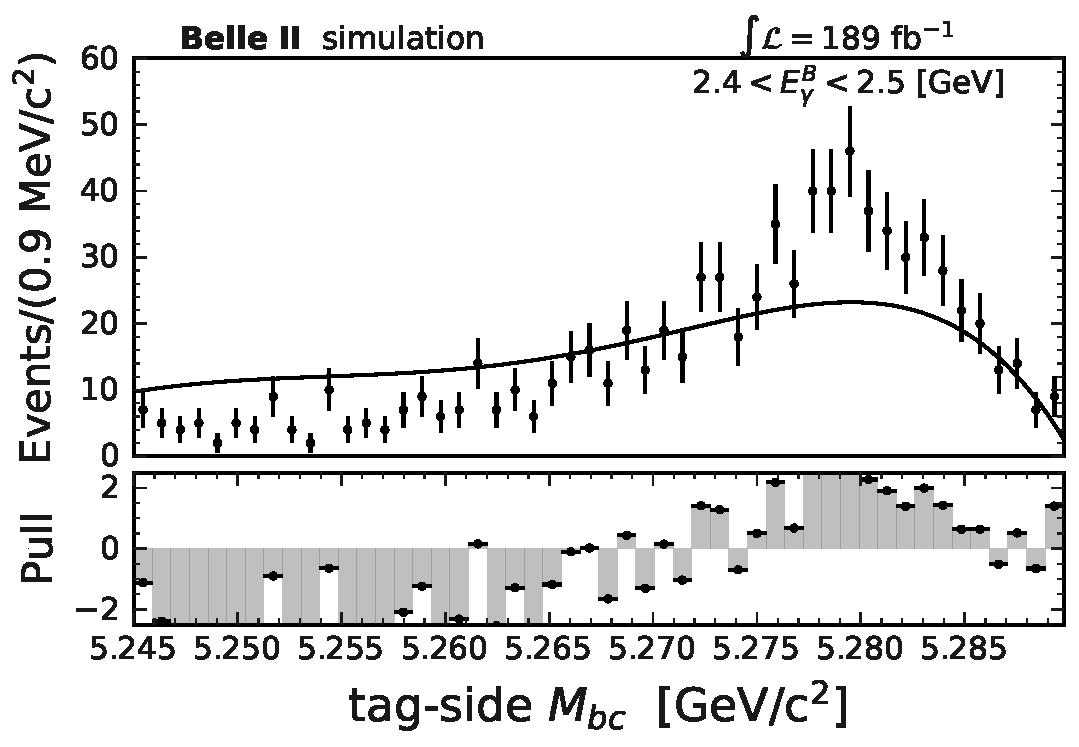
\includegraphics[width=0.3\textwidth]{figures/appendices/primary_fits/CHEB_MbcFit_2p4to2p5ppdf.pdf}
    }
    \subcaptionbox{\label{fig:mbc_cheb_2p5}}{
        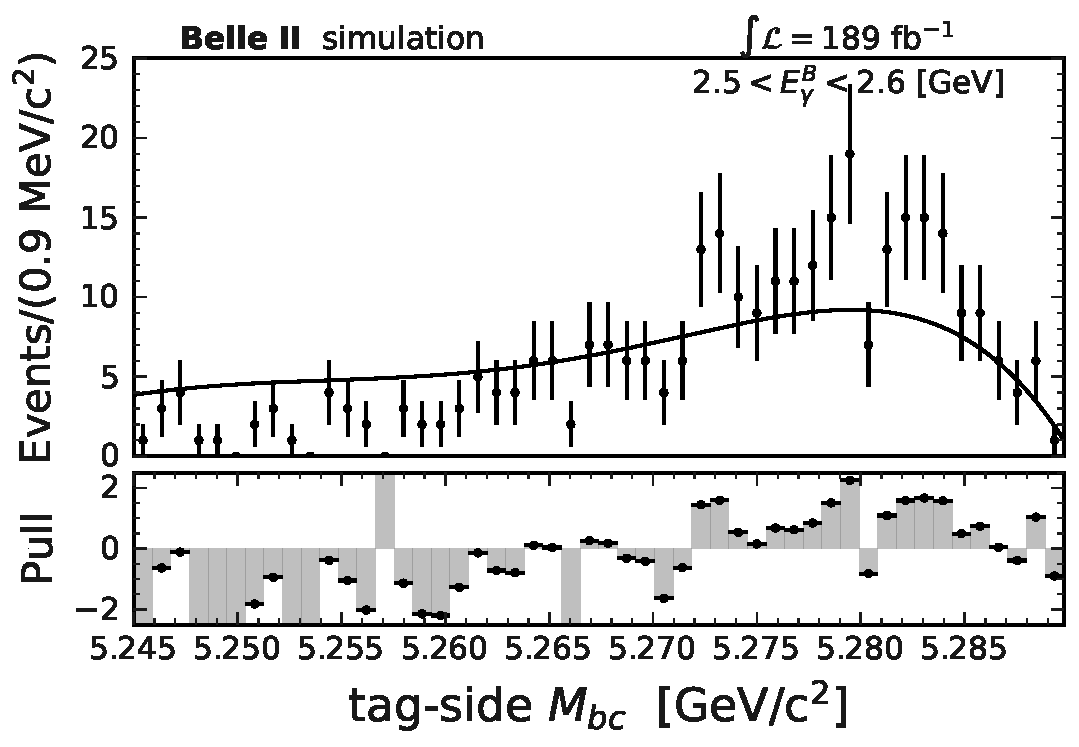
\includegraphics[width=0.3\textwidth]{figures/appendices/primary_fits/CHEB_MbcFit_2p5to2p6ppdf.pdf}
    }
    \subcaptionbox{\label{fig:mbc_cheb_2p6}}{
        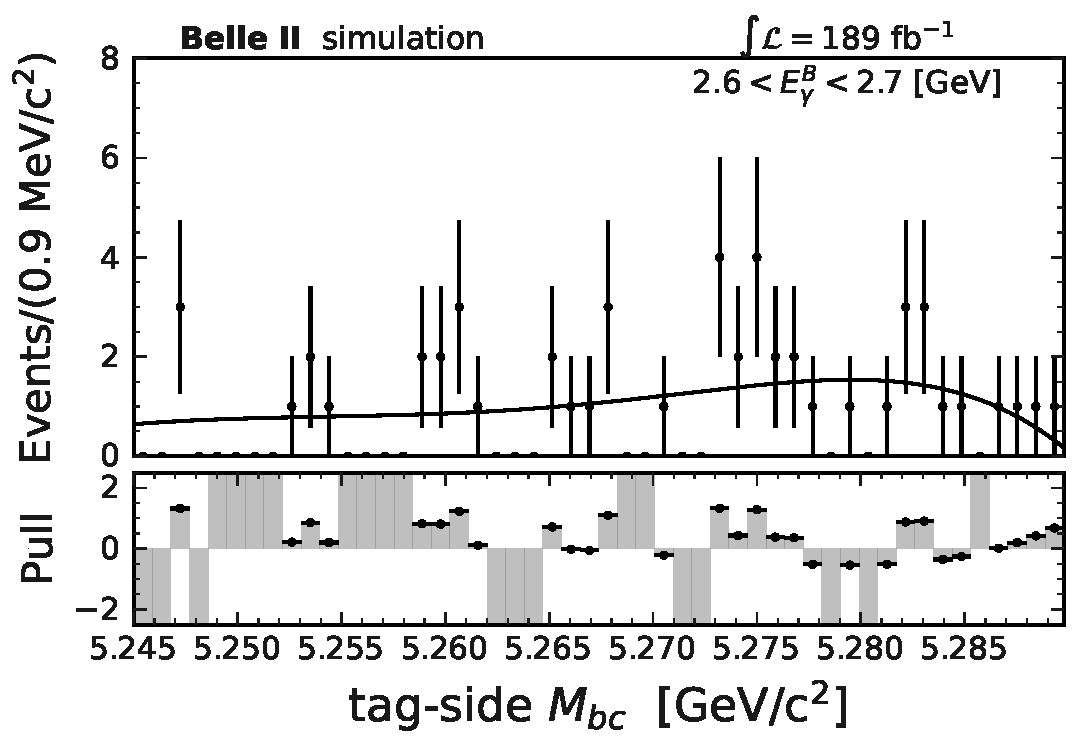
\includegraphics[width=0.3\textwidth]{figures/appendices/primary_fits/CHEB_MbcFit_2p6to2p7ppdf.pdf}
    }
    \subcaptionbox{\label{fig:mbc_cheb_2p7}}{
        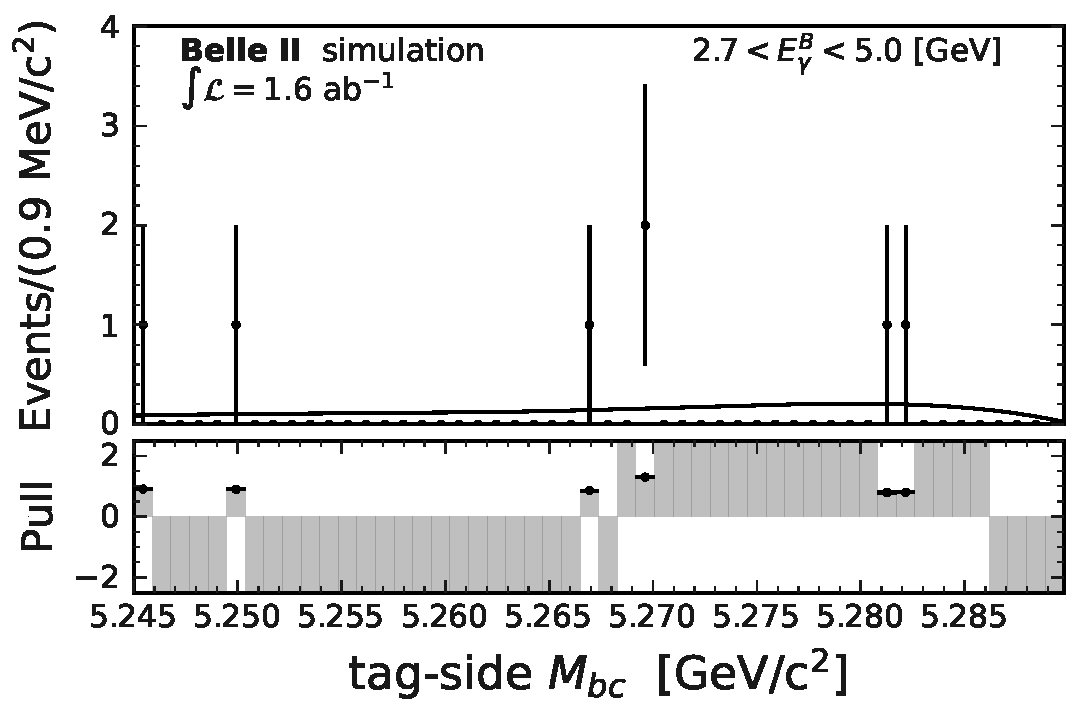
\includegraphics[width=0.3\textwidth]{figures/appendices/primary_fits/CHEB_MbcFit_2p7to5p0ppdf.pdf}
    }
    \caption{\label{fig:primary_cheb_fits}The fits on events with combinatorial-\BB tags in generic \MC, using the Chebyshev \PDF.
    This fit allows to extract initialisation values for further fitting of the total datasets.
    Good description of the \Mbc distributions can be seen throughout the \EB bins.
    }
\end{figure}

\begin{figure}[htbp!]
    \centering
    \subcaptionbox{\label{fig:mbc_bkg_1p4}}{
        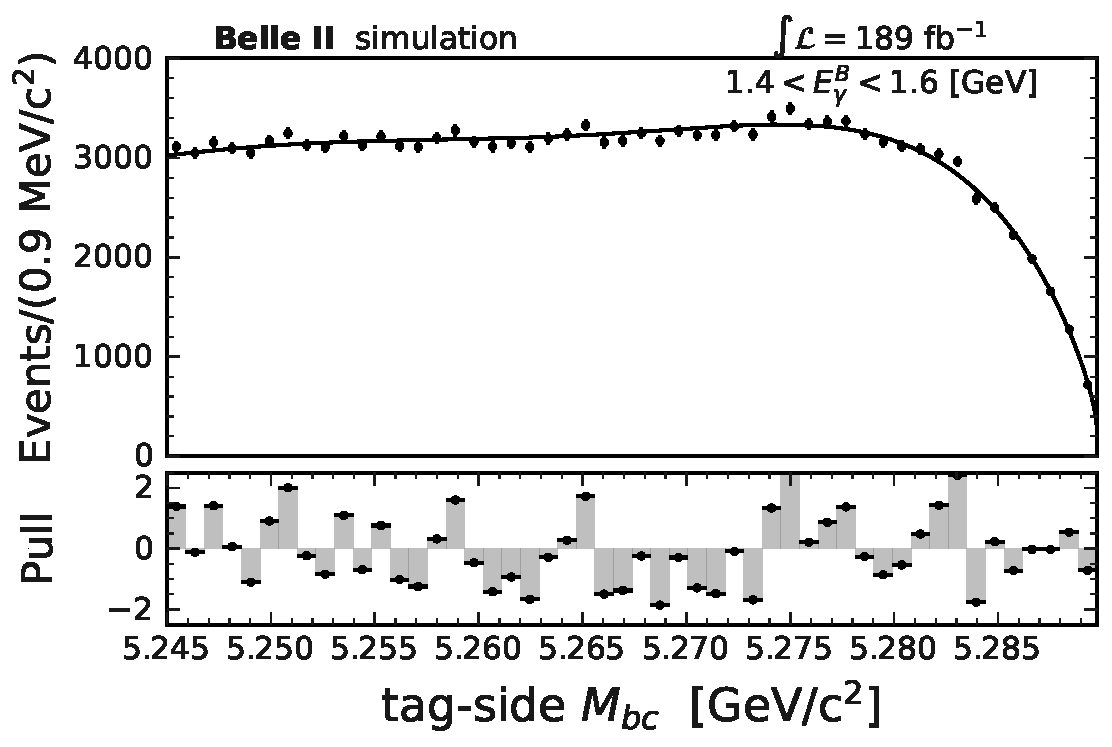
\includegraphics[width=0.3\textwidth]{figures/appendices/primary_fits/BKG_MbcFit_1p4to1p6ppdf.pdf}
    }
    \subcaptionbox{\label{fig:mbc_bkg_1p6}}{
        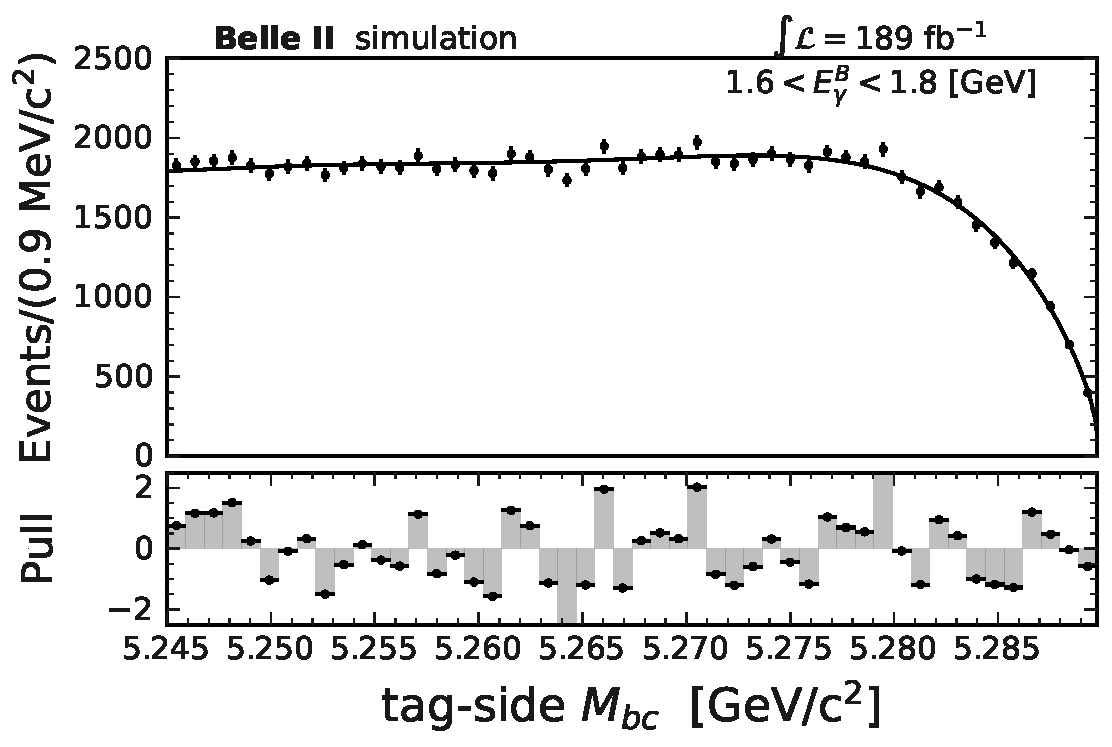
\includegraphics[width=0.3\textwidth]{figures/appendices/primary_fits/BKG_MbcFit_1p6to1p8ppdf.pdf}
    }
    \subcaptionbox{\label{fig:mbc_bkg_1p8}}{
        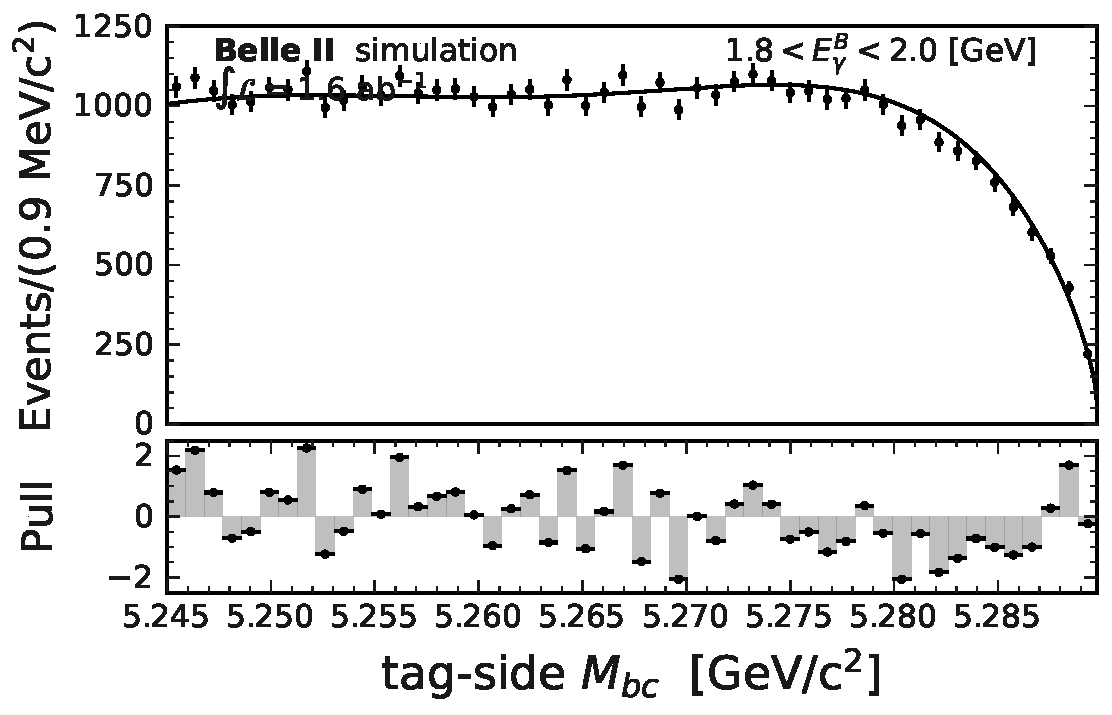
\includegraphics[width=0.3\textwidth]{figures/appendices/primary_fits/BKG_MbcFit_1p8to2p0ppdf.pdf}
    }
    \subcaptionbox{\label{fig:mbc_bkg_2p0}}{
        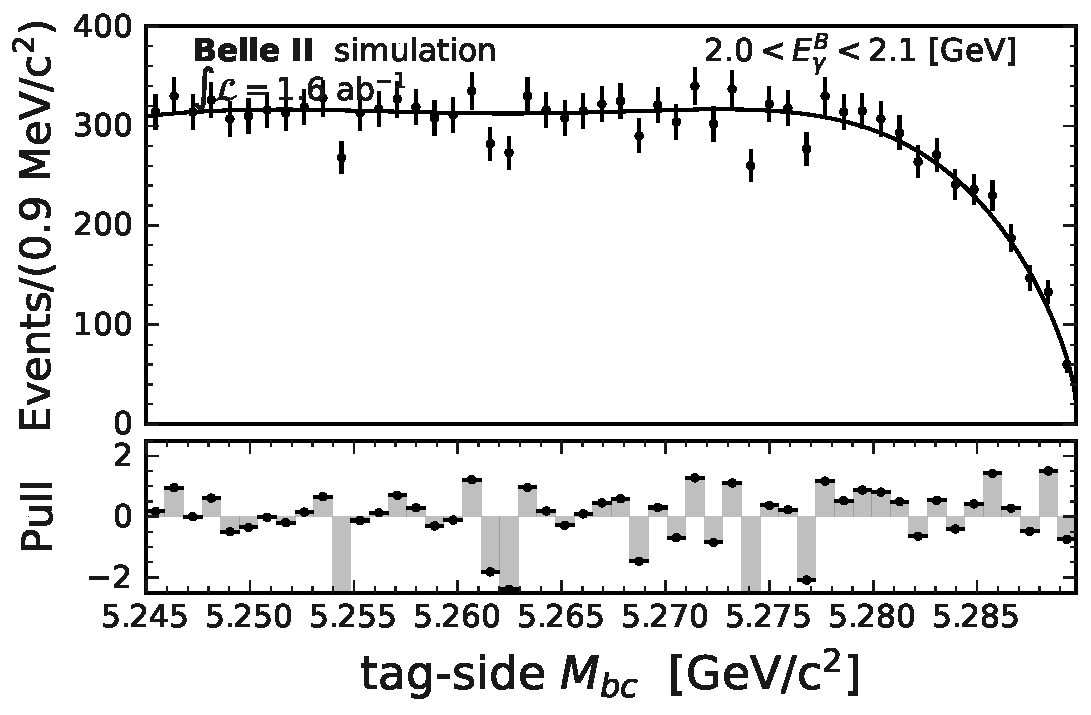
\includegraphics[width=0.3\textwidth]{figures/appendices/primary_fits/BKG_MbcFit_2p0to2p1ppdf.pdf}
    }
    \subcaptionbox{\label{fig:mbc_bkg_2p1}}{
        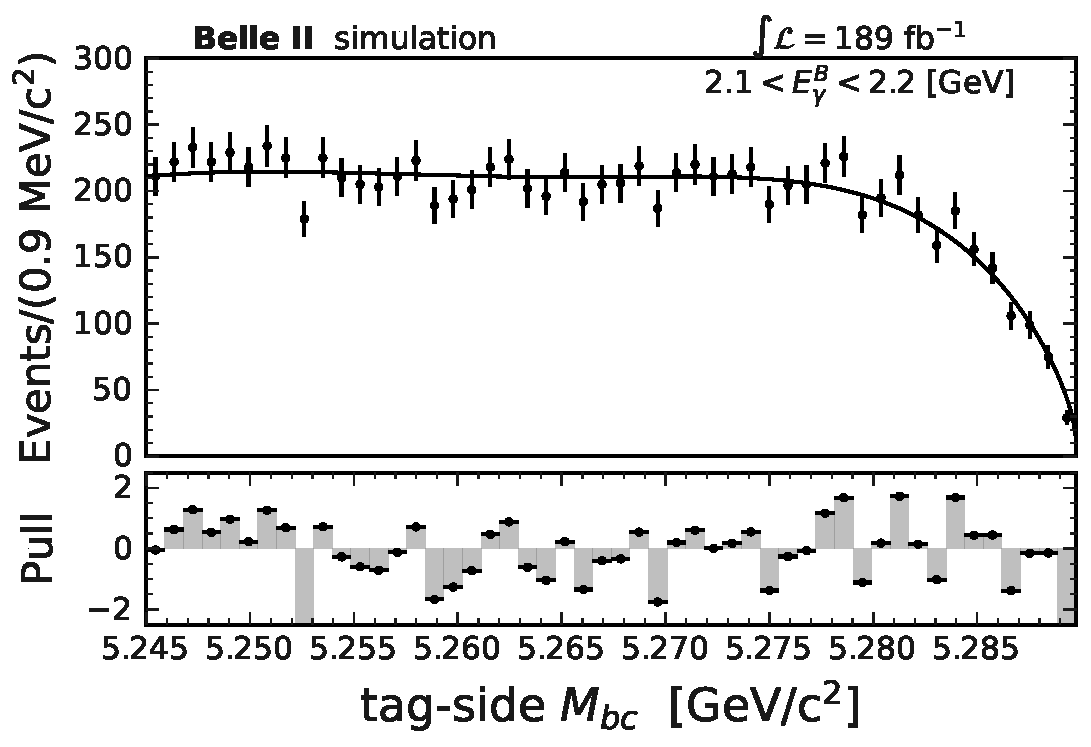
\includegraphics[width=0.3\textwidth]{figures/appendices/primary_fits/BKG_MbcFit_2p1to2p2ppdf.pdf}
    }
    \subcaptionbox{\label{fig:mbc_bkg_2p2}}{
        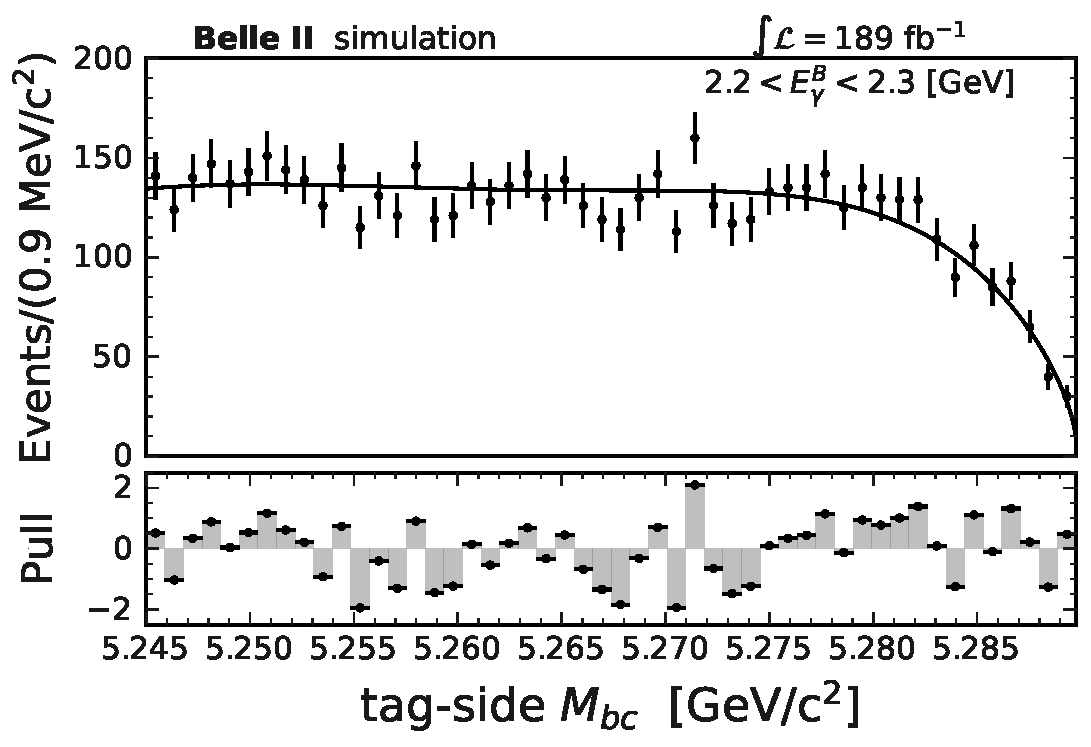
\includegraphics[width=0.3\textwidth]{figures/appendices/primary_fits/BKG_MbcFit_2p2to2p3ppdf.pdf}
    }
    \subcaptionbox{\label{fig:mbc_bkg_2p3}}{
        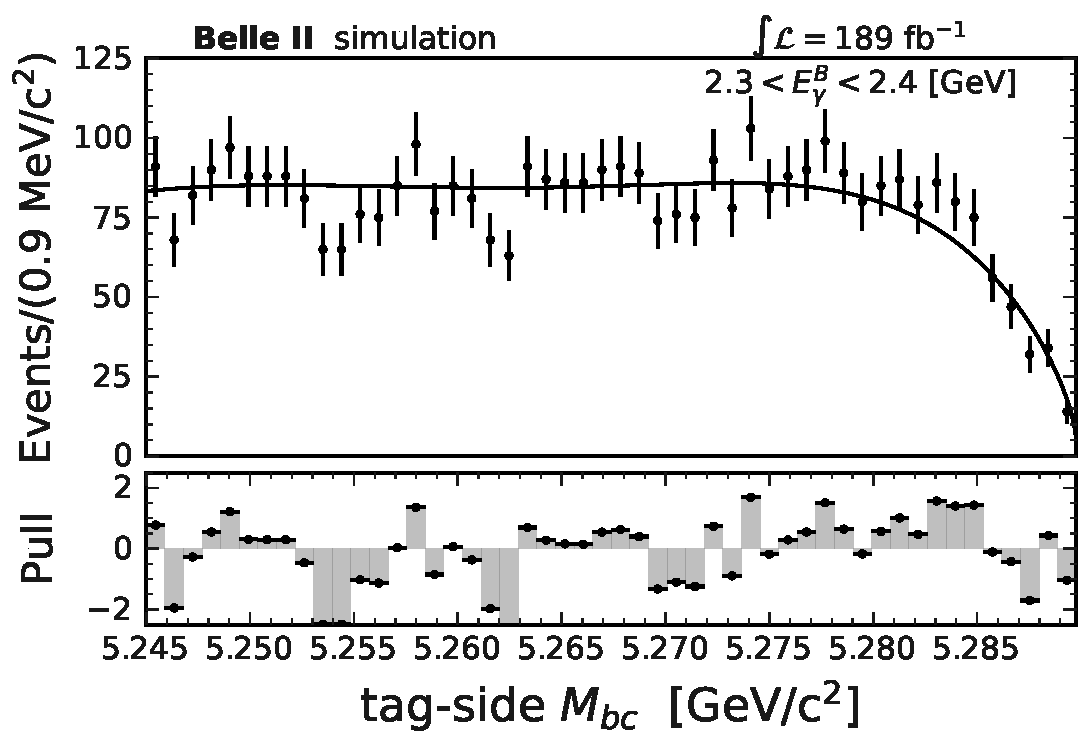
\includegraphics[width=0.3\textwidth]{figures/appendices/primary_fits/BKG_MbcFit_2p3to2p4ppdf.pdf}
    }
    \subcaptionbox{\label{fig:mbc_bkg_2p4}}{
        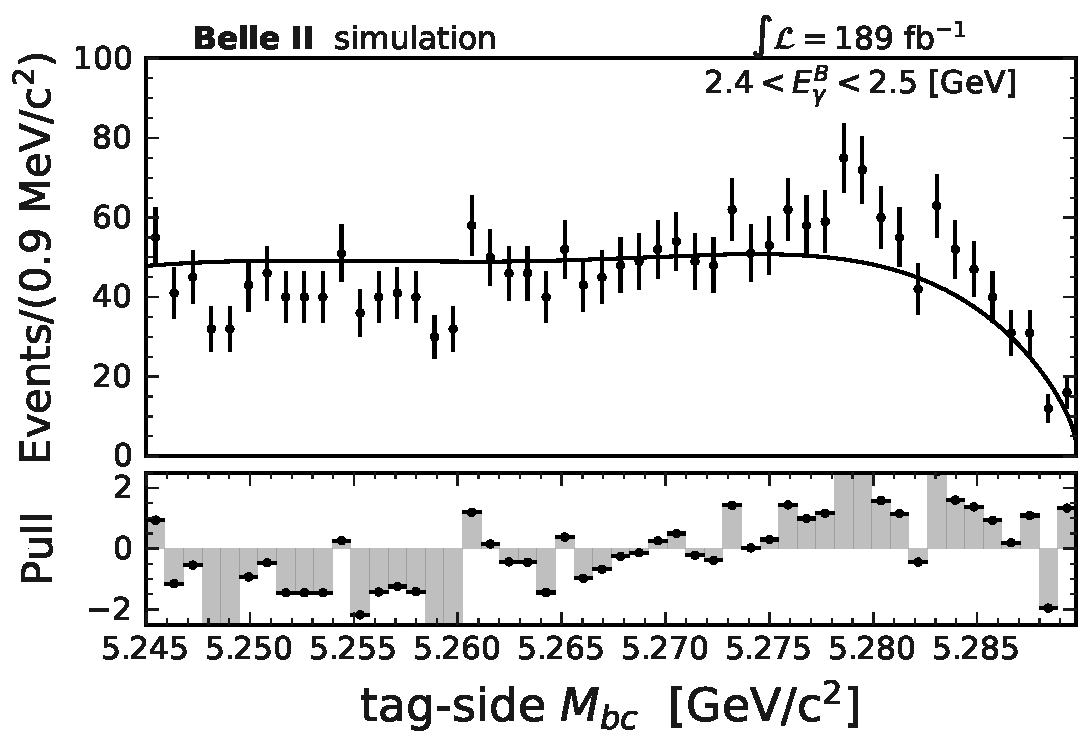
\includegraphics[width=0.3\textwidth]{figures/appendices/primary_fits/BKG_MbcFit_2p4to2p5ppdf.pdf}
    }
    \subcaptionbox{\label{fig:mbc_bkg_2p5}}{
        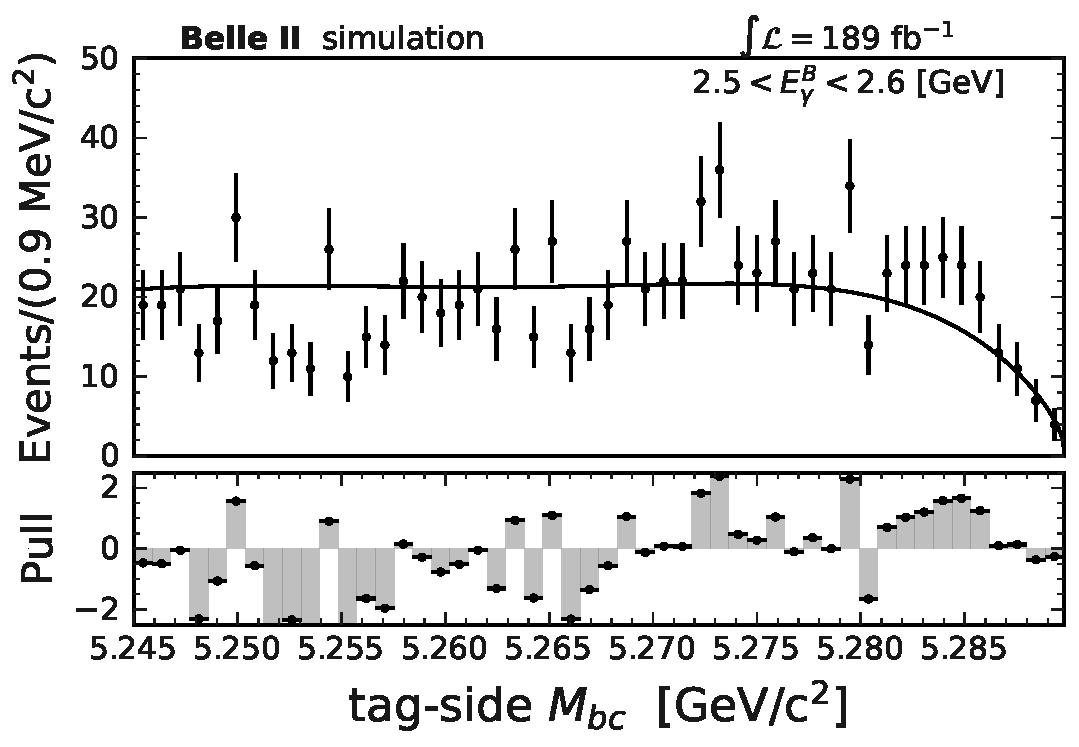
\includegraphics[width=0.3\textwidth]{figures/appendices/primary_fits/BKG_MbcFit_2p5to2p6ppdf.pdf}
    }
    \subcaptionbox{\label{fig:mbc_bkg_2p6}}{
        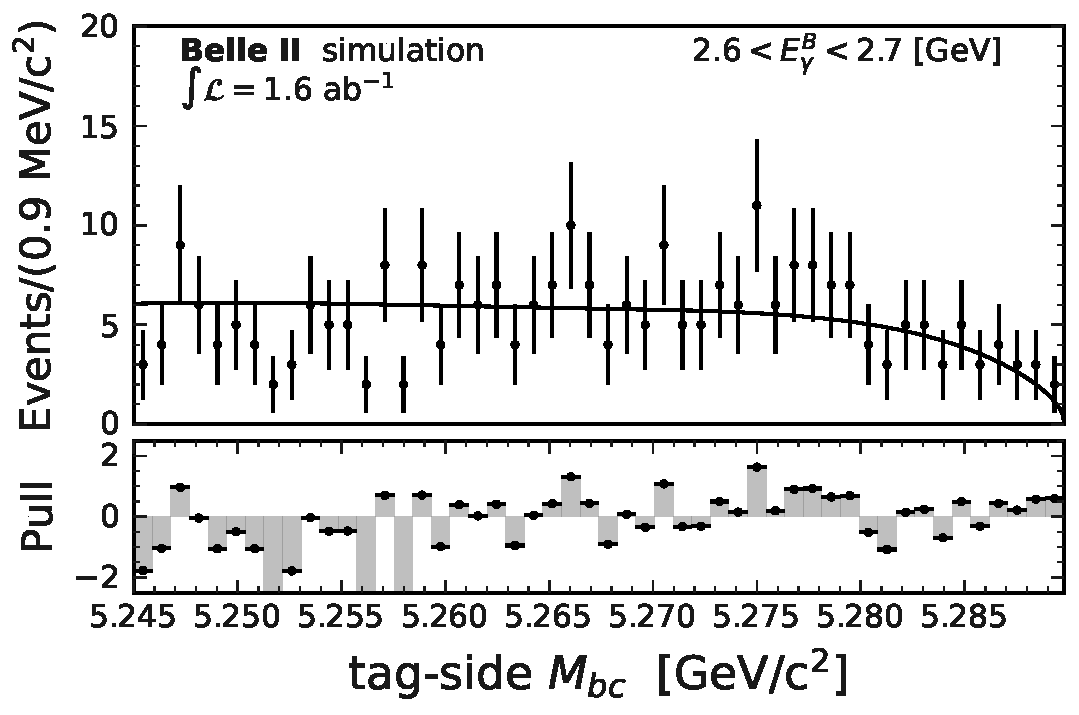
\includegraphics[width=0.3\textwidth]{figures/appendices/primary_fits/BKG_MbcFit_2p6to2p7ppdf.pdf}
    }
    \subcaptionbox{\label{fig:mbc_bkg_2p7}}{
        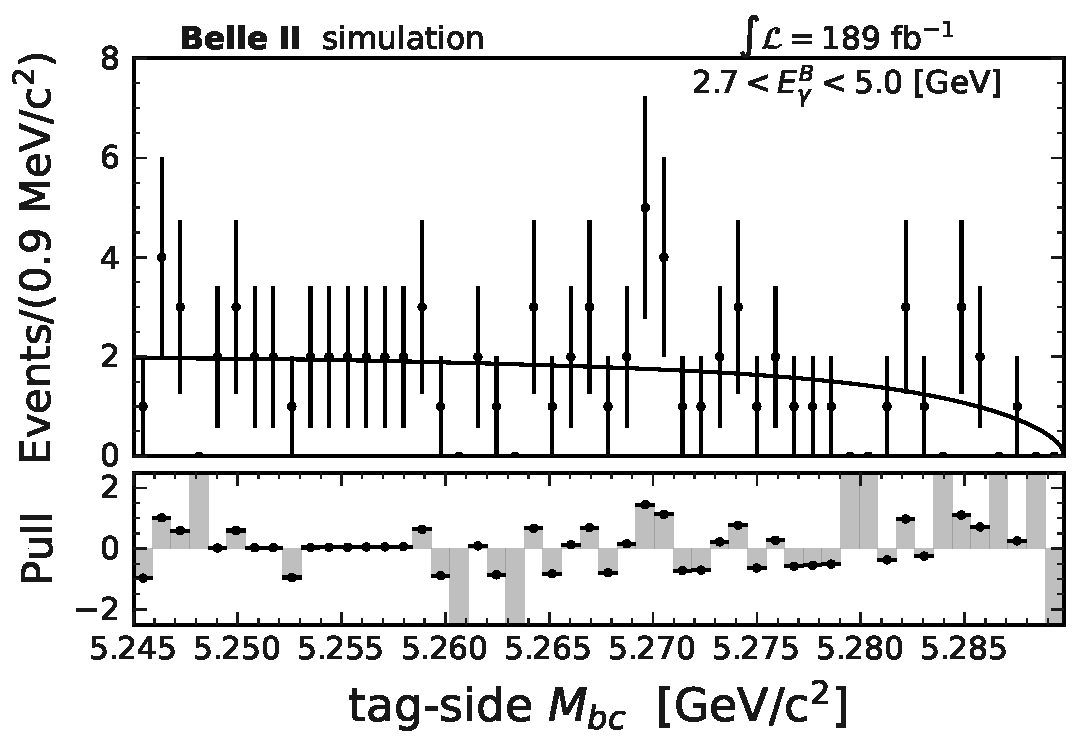
\includegraphics[width=0.3\textwidth]{figures/appendices/primary_fits/BKG_MbcFit_2p7to5p0ppdf.pdf}
    }
    \caption{\label{fig:primary_bkg_fits}The combined fits from \Cref{fig:primary_argus_fits,fig:primary_cheb_fits} visualised on the combined combinatorial-\BB tag and continuum event datasets in generic \MC.
    An excellent overall description of the \Mbc distributions can be seen, especially taking into account that the Belle II dataset for this analysis is roughly one order of magnitude smaller than the amount of simulated data fit here.
    }
\end{figure}